\addtocontents{toc}{\protect\newpage}
\chapter[Persistent Homology for Amorphous Materials]{Persistent Homology for \\ Amorphous Materials}
\label{ch:ph}

\begin{chapterabstract}
Persistent homology is a technique in topological data analysis to find the fundamental topological features collections of points.
The applicability of persistent homology to the characterisation of network materials is explored here for the relatively simple case of \td{} networks. 
Analysis is carried out for two systems, triangle rafts and continuous random networks (CRNs), which have different underlying constraints.
The persistence diagrams of triangle rafts are shown to have a band structure which originates in successive nearest\--neighbour interactions, whilst the evolution of Betti numbers is related to the underlying ring statistics.
These are compared and contrasted with CRNs, which display broader and more aggregated persistence diagrams.
Conclusions are drawn of relevance to more complex systems.
\end{chapterabstract}

\section{Introduction to Persistent Homology}

The need for efficient methods to find structure in large and complex data sets is ever increasing in the age of ``big data''.
The field of topological data analysis (TDA) has emerged to address this need, driving the development of statistical tools to analyse and understand big, noisy, real\--world data \cite{Wasserman2018}.
One tool in particular has received significant attention, namely that of persistent homology \cite{Edelsbrunner2008}.
Persistent homology is concerned with finding the fundamental topological features in a given set of points. 
In slightly plainer terms, here \textit{homology} means counting the number of connected components and cycles  in a system.
The persistence aspect arises from the fact that the these topological features can be calculated across different length scales, with those existing across multiple length scales being identified as more \textit{persistent}.
The more persistent a topological feature, the more it can be thought of as reflecting the true underlying system topology.

%As with any new technique which arrives with much fanfare, persistent homology has been quickly appropriated for the study of chemical and physical systems.
%In fact, the marriage of persistent homology and atomistic materials seems apt.
The application of persistent homology to atomistic materials seems appropriate.
Atomic systems have long been thought of in terms of collections of point like particles, and the study of the emergent structure is deep\--rooted in the field.
Any process which can elucidate as yet hidden structure in materials, or improve its description naturally has potential to be extremely useful.
In this vein, research has already been conducted on applying persistent homology to diverse topics such as colloidal packings \cite{Carter2018}, porous media \cite{Robins2017,Jiang2018}, water networks \cite{Steinberg2019}, fullerenes \cite{Xia2015}, and of particular importance to this work, amorphous materials \cite{Hiraoka2016,Onodera2019,Nakamura2015,Gutierrez2019}.
Whilst these latter studies claim to highlight structures which are not available using more conventional techniques, quantify the medium range order in glasses, and explain phenomena such as the origin of the first sharp diffraction peak in disordered materials; the fact remains that persistent homology remains a qualitative descriptor, with some doubt as to what is the ``added value'' from this technique. 
In the words of Wassserman: ``\textit{...the main purpose of TDA is to help the data analyst summarize and visualize
complex datasets. Whether or not TDA can be used to make scientific discoveries is still unclear.}'' \cite{Wasserman2018}.

The purpose of this chapter is therefore to try and assess the utility of persistent homology in the context of \td{} amorphous materials, with the expectation that the interpretation may be simpler for these reduced dimensionality systems.
%The conclusions drawn from this work may then bring insight to the analysis of three dimensional systems.
This chapter will begin by outlining the relevant theory to persistent homology, with the aid of small example systems.
Persistent homology will then be calculated for triangle rafts (a proxy for amorphous silica), systematically generated with increasing levels of disorder.
These results will then be contrasted with generic continuous random networks (CRNs) as produced from bond switching.
Finally, the conclusions of these investigations will be discussed in the context of more complex systems, and the potential usefulness of persistent homology as an analytic tool for materials examined.

\section{Computing Persistent Homology}

This section will give a broad outline of the mathematical background behind persistent homology, but with the focus on a practicable implementation for studying physical \td{} networks.
It will begin by introducing the concept of a filtered simplicial complex, before discussing homology groups, persistent homology and the visualisation of persistence.
These principles will be applied to small example crystalline and amorphous configurations.
Actual numerical persistent homology calculations are carried out with the GUDHI library \cite{gudhi}.

\subsection{Filtered Simplicial Complexes}

The input for a persistent homology calculation is simply a point cloud \ie{} a set of coordinates in Euclidean space.
For materials, this corresponds to the set of atomic positions, $\mathbf{r}=\left\{r_1,r_2,\cdots,r_\mathcal{N}\right\}$, as obtained from simulation or from experimental microscopy.
Using this point cloud, a filtered simplicial complex can be constructed \cite{Fugacci2016}.
To explain what is meant by a filtered simplicial complex, it is useful to break down this definition further:
\begin{itemize}
	\item An $m$\--simplex, $\sigma$, is a subset of the total points, $\sigma\subseteq\mathbf{r}$, with dimension $m=\abs{\sigma}-1$.
Put simply, a $0$\--simplex corresponds to a point, a $1$\--simplex to a line, a $2$\--simplex a triangle, a $3$\--simplex a tetrahedron, and so on.% and so forth.
	\item A simplicial complex, $\mathbf{K}$, is then a set of simplices, $\mathbf{K}=\left\{\sigma_1,\sigma_2,\dots\right\}$.
	\item A filtration of a simplicial complex, is a sequence of subcomplexes: $\mathbf{K}_a \subseteq \mathbf{K}_b \subseteq \cdots \subseteq \mathbf{K}$, where each subcomplex, $\mathbf{K}_\epsilon$, occurs at an increasing filtration value, denoted $\epsilon$ (see below).
\end{itemize}
For a given point cloud, there are many ways to then construct a filtered simplicial complex (Cech, Vietoris\--Rips, Witness \etc), each method identifying simplices and calculating filtration values in a different manner  \cite{Otter2017}.
In this thesis, for reasons which will become apparent, the \textit{alpha complex} is used.

\begin{figure}[tb]
	\centering
     
	\begin{subfigure}[b]{0.45\textwidth}
         \centering
         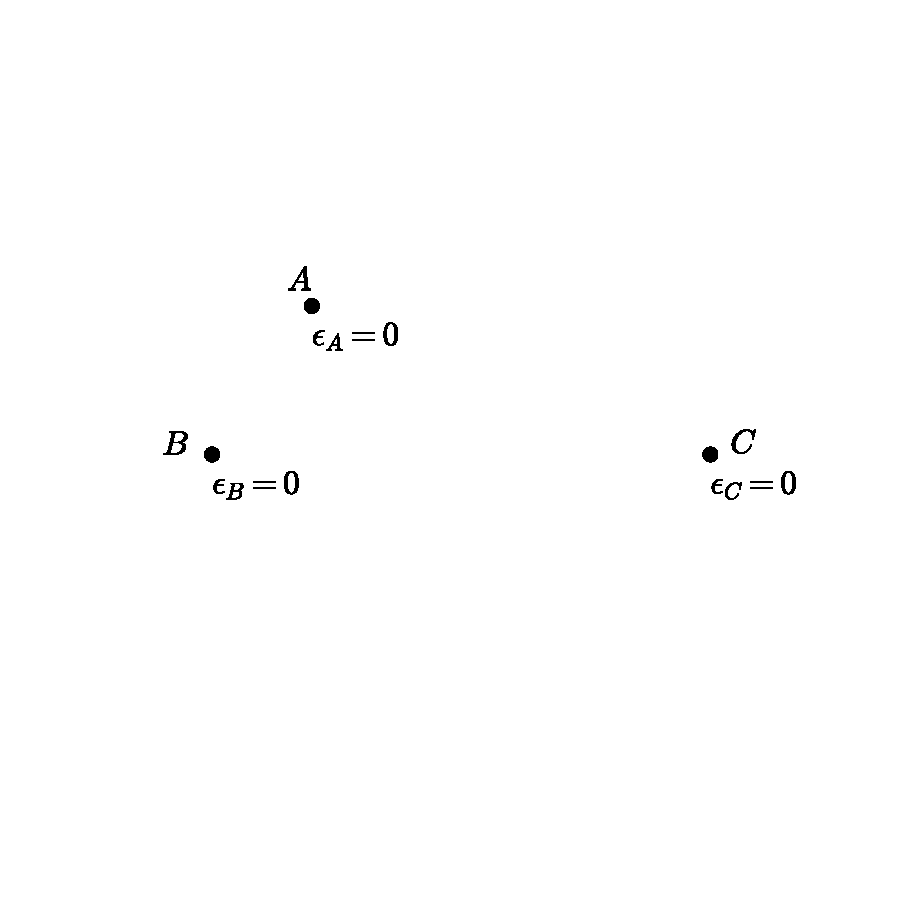
\includegraphics[width=\textwidth]{./figures/ph/alpha_a.pdf}
          \caption{$\sigma_1=\left\{A\right\}$, $\sigma_2=\left\{B\right\}$, $\sigma_3=\left\{C\right\}$; \\ $\mathbf{K}_0 = \left\{\sigma_1,\sigma_2,\sigma_3\right\}$}
         \label{fig:phalphaa}
     \end{subfigure}
     \hfill  
       \begin{subfigure}[b]{0.45\textwidth}
         \centering
         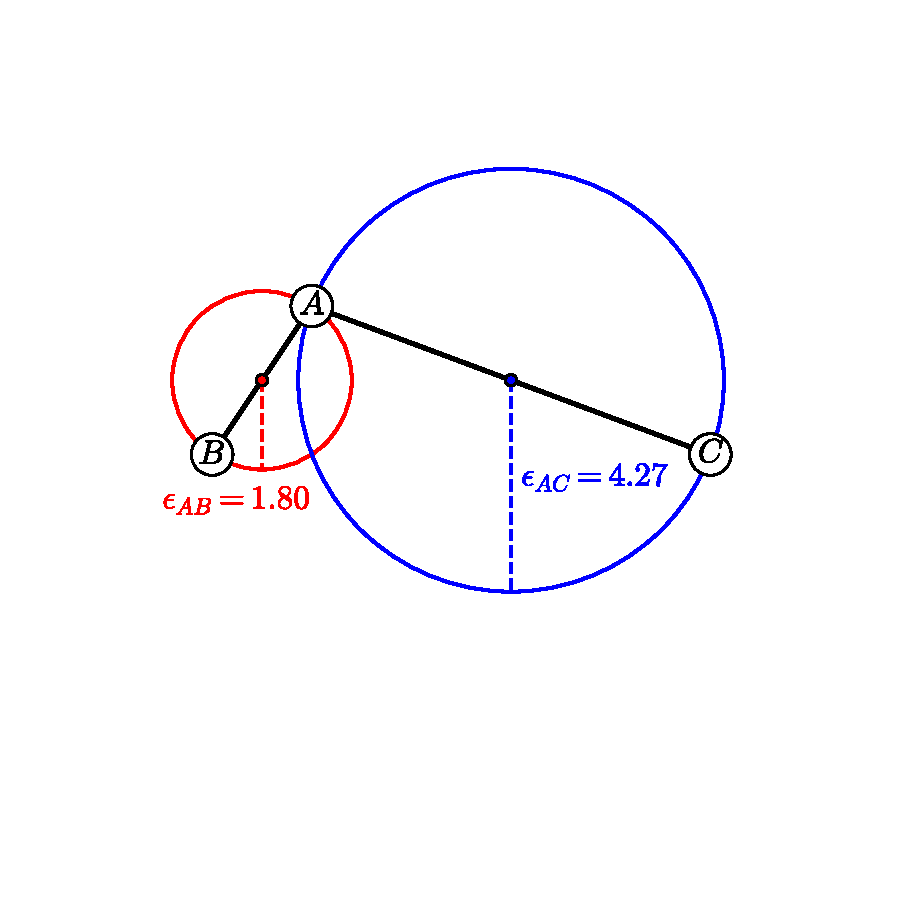
\includegraphics[width=\textwidth]{./figures/ph/alpha_b2.pdf}
        \caption{$\sigma_4=\left\{A,B\right\}$, $\sigma_5=\left\{A,C\right\}$; \\ $\mathbf{K}_{4.27} = \left\{\sigma_1,\sigma_2,\cdots,\sigma_5\right\}$}
         \label{fig:phalphab1}
     \end{subfigure}
     \hfill
        
      \vspace{0.5cm}
      \begin{subfigure}[b]{0.45\textwidth}
         \centering
         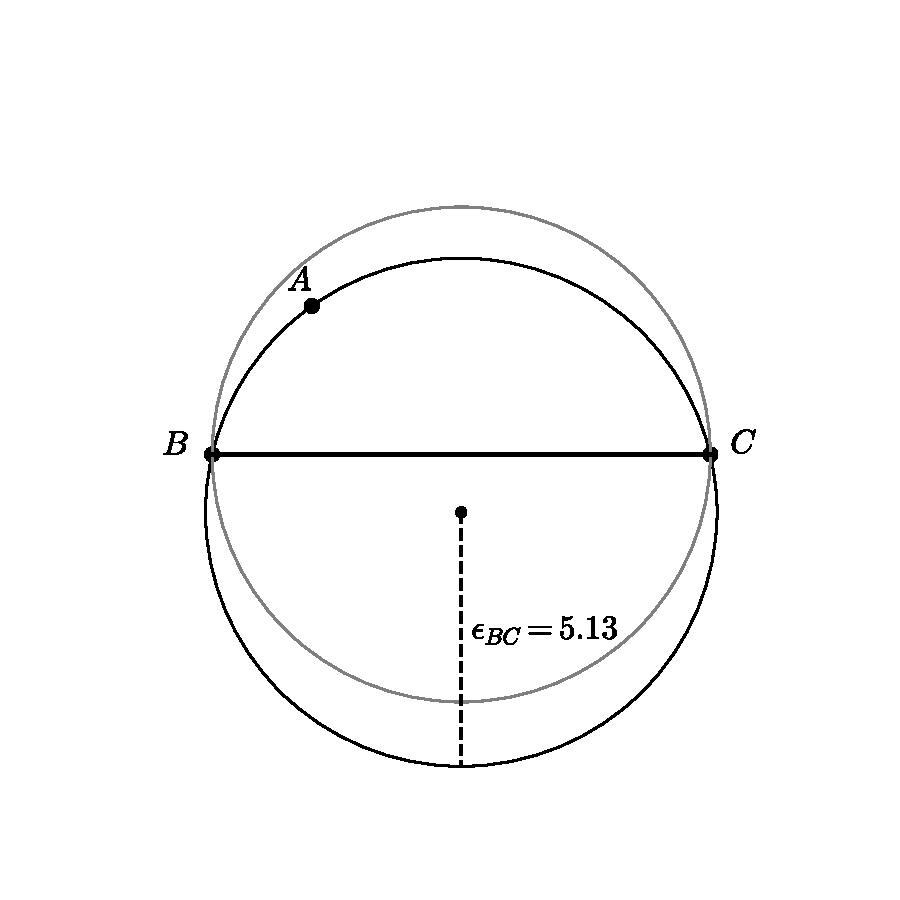
\includegraphics[width=0.85\textwidth]{./figures/ph/alpha_b1.pdf}
         \caption{$\sigma_6=\left\{B,C\right\}$ \\ \phantom{x}}
         \label{fig:phalphab2}
     \end{subfigure}
     \hfill
      \begin{subfigure}[b]{0.45\textwidth}
         \centering
         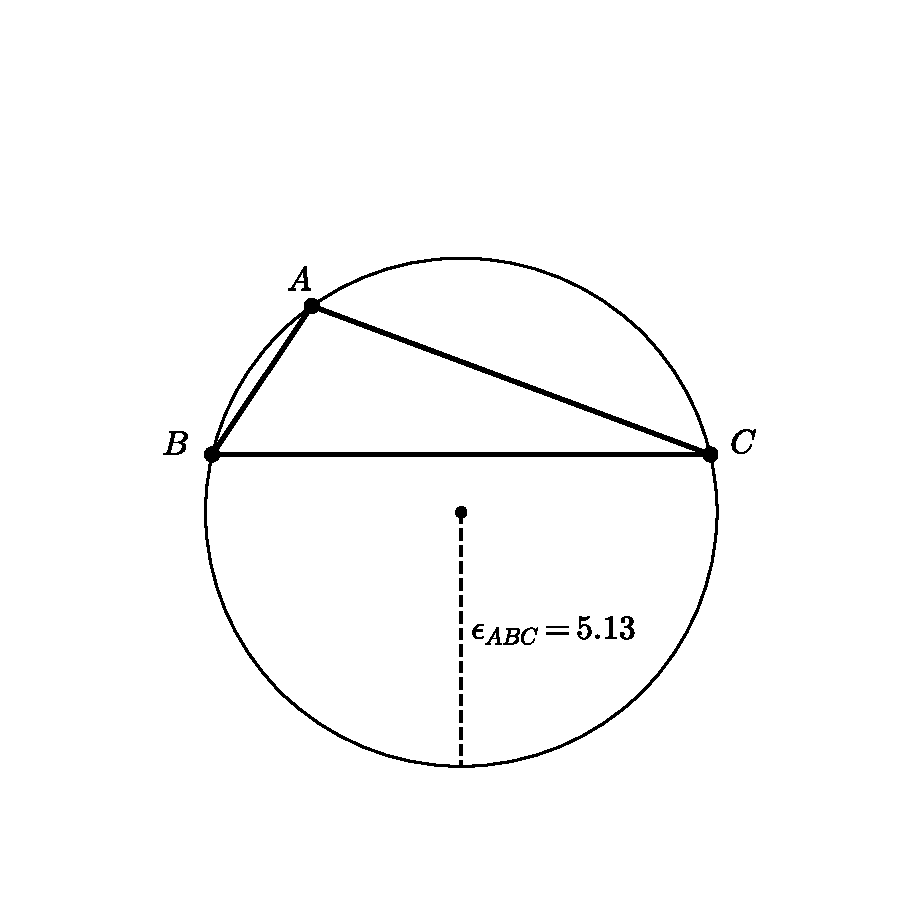
\includegraphics[width=0.85\textwidth]{./figures/ph/alpha_c.pdf}
         \caption{$\sigma_7=\left\{A,B,C\right\}$; \\ $\mathbf{K}_{5.13}=\mathbf{K}_{\infty} = \left\{\sigma_1,\sigma_2,\cdots,\sigma_7\right\}$}
         \label{fig:phalphac}
     \end{subfigure}
     \hfill
    
	\caption{Construction of an alpha simplicial complex and its filtration. Panel (a) shows three 0\--simplices, with filtration values of $\epsilon=0$. Panel (b) shows an additional two 1\--simplices, with filtration values given by the radii of the respective circumcircles (dashed lines in circles). Panel (c) shows an additional different 1\--simplex, in which the circumcircle (red circle) contains the 2\--simplex $\left\{A,B,C\right\}$, and so the filtration value is set to the value of the 2\--simplex. Panel (d) shows the 2\--simplex with a filtration value given by the circumradius.
	These subfigures can also be viewed as a series of subcomplexes, as highlighted in the captions, with $\mathbf{K}_0\subseteq\mathbf{K}_{4.27}\subseteq\mathbf{K}_{5.13}=\mathbf{K}_\infty$. The final complex is the Delaunay triangulation of the original point set. Panel (c) is \textit{not} a subcomplex in the filtration, as it does not contain the simplices $\left\{A,B\right\}$, $\left\{A,C\right\}$, which have lower filtration values than $\left\{B,C\right\}$. }
	\label{fig:phalpha}
\end{figure}

To illustrate these concepts, an introductory example with just three points is given in figure \ref{fig:phalpha}.
Considering only the simplices at first: figure \ref{fig:phalphaa} contains three 0\--simplices, the points $A$, $B$, $C$; figures \ref{fig:phalphab1} and \ref{fig:phalphab2} three 1\--simplices, the lines $AB$, $AC$, $BC$; figure \ref{fig:phalphac} a 2\--simplex, the triangle $ABC$.
Once the simplices have been identified, a filtration value, $\epsilon$, is computed and assigned to each.
For the alpha complex, filtration values are determined from the radius of the circumcircles containing the simplices.
The specific algorithm is as follows:
\begin{itemize}
	\item 0\--simplices: have a filtration value of $\epsilon=0$.
	\item 1\--simplices: provided the circumcircle is empty, they have a filtration value equal to its radius, which for two points is equivalent to half the line length $\epsilon=r_{ij}/2$.
	If the circumcircle contains a 2\--simplex, then the filtration value is set to the filtration value of that simplex.
	\item 2\--simplices: have a filtration value equal to the circumradius.
\end{itemize}
These different cases are shown and explained in figure \ref{fig:phalpha}.

Having calculated the filtration values for each simplex, a subcomplex can be generated, $\mathbf{K}_\epsilon$, which contains only the simplices with filtration values less than or equal to $\epsilon$.
Finally, the filtered simplicial complex emerges as a sequence of subcomplexes at increasing filtration values from $\epsilon=0\rightarrow \infty$.
Again figure \ref{fig:phalpha} shows this process for the case of three points.
The first subcomplex, $\mathbf{K}_0$, will only consist of a set of discrete points (as in figure \ref{fig:phalphaa}).
As the filtration value increases, higher dimensionality simplices will be included, as lines and triangles form (as in figure \ref{fig:phalphab1}).
The last subcomplex, $\mathbf{K}_\infty$, will contain all the determined simplices (as in figure \ref{fig:phalphac}).
Crucially, for the alpha complex, this will be equivalent to the Delaunay triangulation.
This is the motivation for choosing the alpha complex, as the Delaunay triangulation (which has already appeared throughout this thesis as the dual of the Voronoi diagram), is well defined in two dimensions. 
As such it provides the best opportunity to relate the results of persistent homology to well understood systems.

\subsection{Homology and Persistent Homology}

Having introduced the notion of a filtered simplicial complex, the importance of homology and persistent homology can now be discussed.
To facilitate this, two more involved examples will be used.
Figures \ref{fig:phexa}\--\ref{fig:phexd} and \ref{fig:phexe}\--\ref{fig:phexh} show filtrations of alpha complexes for a crystalline and an amorphous atomic configuration respectively, which will be referred to throughout this section.

\begin{figure}[tb]
	\centering
     
      \begin{subfigure}[b]{0.22\textwidth}
         \centering
         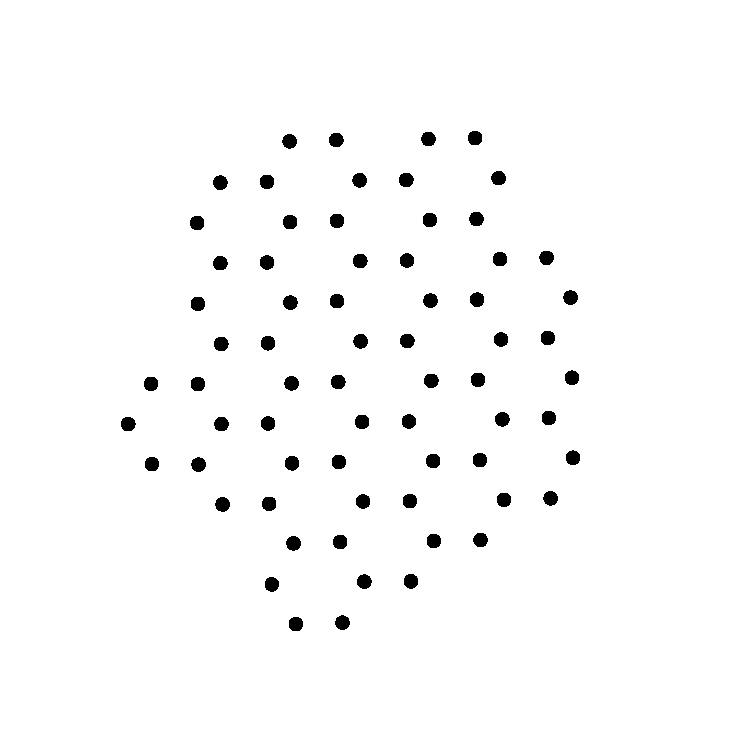
\includegraphics[width=\textwidth]{./figures/ph/ph_ex_crys_0.pdf}
         \caption{$\mathbf{K}_0$,\\ $\beta_0=68$, $\beta_1=0$}
         \label{fig:phexa}
     \end{subfigure}
     \hfill
      \begin{subfigure}[b]{0.22\textwidth}
         \centering
         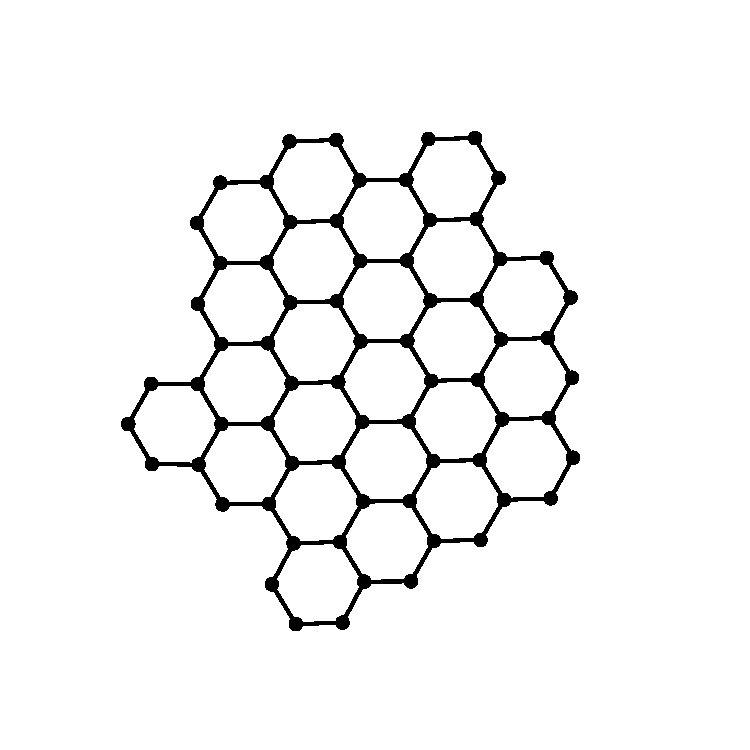
\includegraphics[width=\textwidth]{./figures/ph/ph_ex_crys_12.pdf}
         \caption{$\mathbf{K}_{0.55}$,\\ $\beta_0=1$, $\beta_1=24$}
         \label{fig:phexb}
     \end{subfigure}
     \hfill
     \begin{subfigure}[b]{0.22\textwidth}
         \centering
         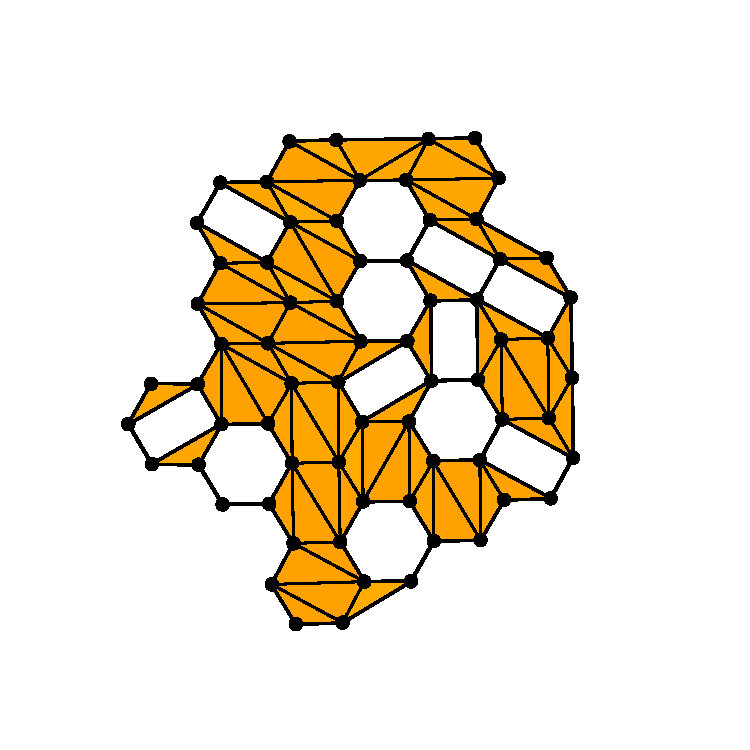
\includegraphics[width=\textwidth]{./figures/ph/ph_ex_crys_20.pdf}
         \caption{$\mathbf{K}_{0.99}$,\\ $\beta_0=1$, $\beta_1=12$}
         \label{fig:phexc}
     \end{subfigure}
     \hfill
     \begin{subfigure}[b]{0.22\textwidth}
         \centering
         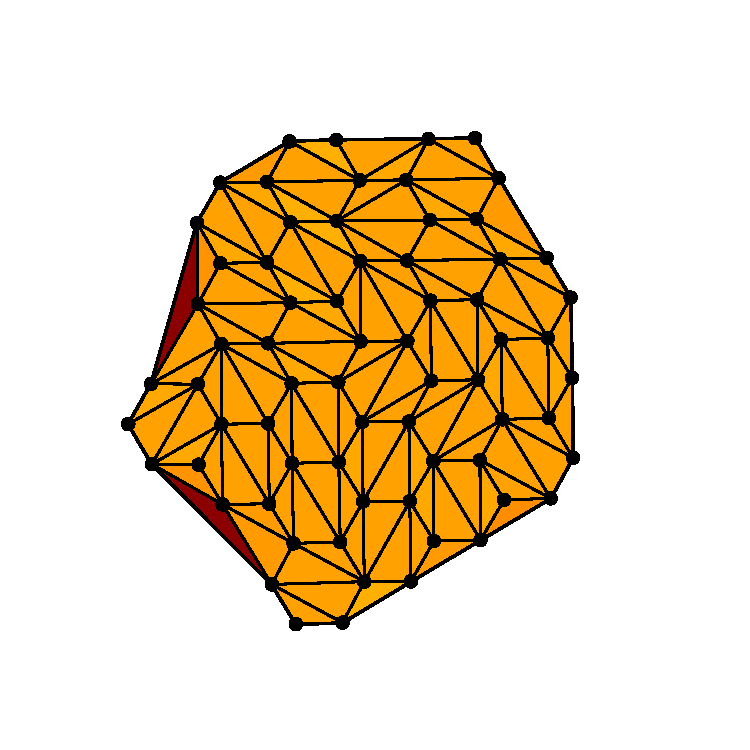
\includegraphics[width=\textwidth]{./figures/ph/ph_ex_crys_inf.pdf}
         \caption{$\mathbf{K}_\infty$,\\ $\beta_0=1$, $\beta_1=0$}
         \label{fig:phexd}
     \end{subfigure}
     
     \vspace{0.5cm}
     \begin{subfigure}[b]{0.22\textwidth}
         \centering
         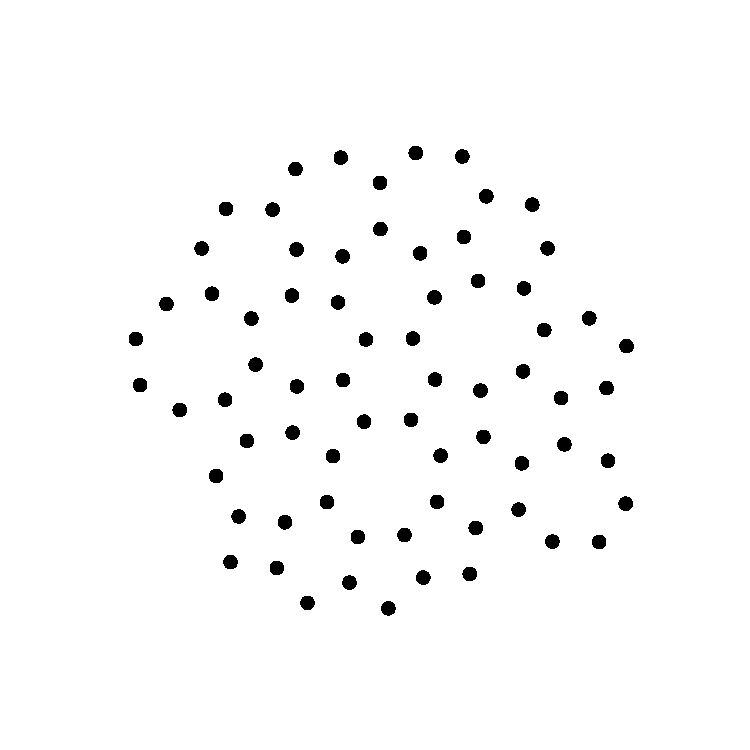
\includegraphics[width=\textwidth]{./figures/ph/ph_ex_amorph_0.pdf}
         \caption{$\mathbf{K}_0$,\\ $\beta_0=70$, $\beta_1=0$}
         \label{fig:phexe}
     \end{subfigure}
     \hfill
      \begin{subfigure}[b]{0.22\textwidth}
         \centering
         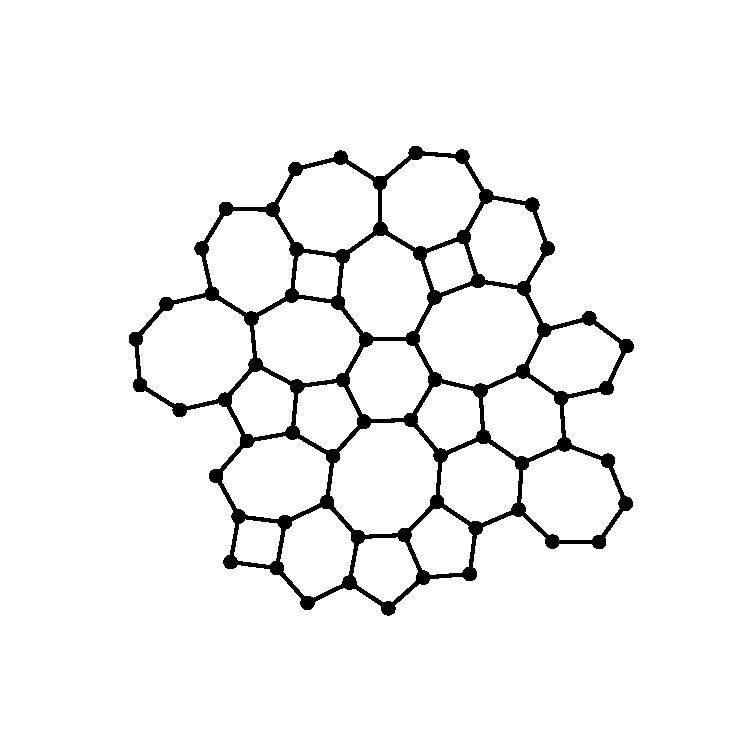
\includegraphics[width=\textwidth]{./figures/ph/ph_ex_amorph_12.pdf}
         \caption{$\mathbf{K}_{0.55}$,\\ $\beta_0=1$, $\beta_1=24$}
         \label{fig:phexf}
     \end{subfigure}
       \hfill
      \begin{subfigure}[b]{0.22\textwidth}
         \centering
         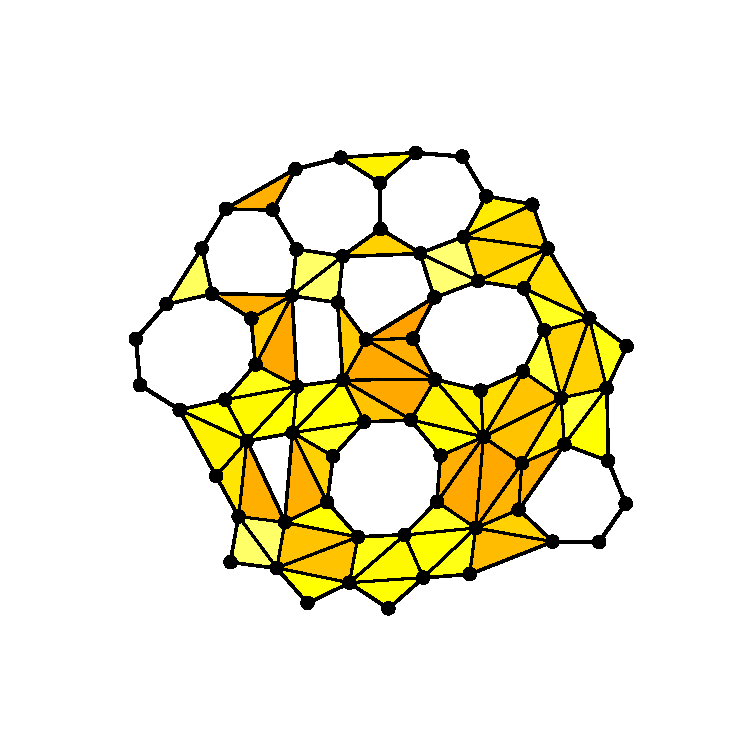
\includegraphics[width=\textwidth]{./figures/ph/ph_ex_amorph_20.pdf}
         \caption{$\mathbf{K}_{0.99}$,\\ $\beta_0=1$, $\beta_1=10$}
         \label{fig:phexg}
     \end{subfigure}
       \hfill
      \begin{subfigure}[b]{0.22\textwidth}
         \centering
         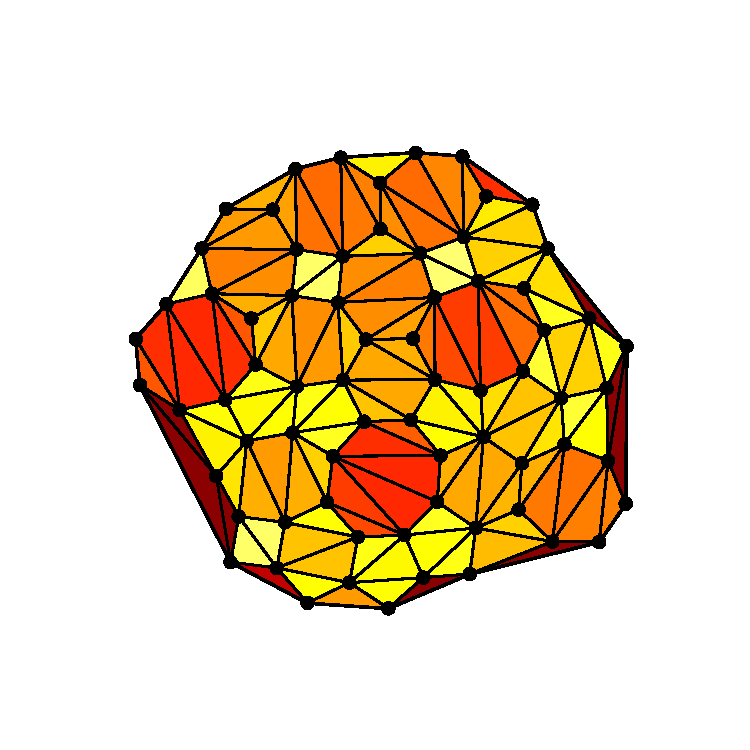
\includegraphics[width=\textwidth]{./figures/ph/ph_ex_amorph_inf.pdf}
         \caption{$\mathbf{K}_\infty$,\\ $\beta_0=1$, $\beta_1=0$}
         \label{fig:phexh}
     \end{subfigure}
   
	\caption{Filtered alpha complexes for a crystalline (panels (a)\--(d)) and amorphous (panels (e)\--(h)) configuration. The Betti numbers for the 0\-- and 1\--dimensional features are also given in the captions, corresponding to the number of connected components and cycles respectively. In addition 2\--simplices are coloured according to their filtration value, with yellow$\rightarrow$red indicating a larger filtration value. This highlights that all 2\--simplices form almost simultaneously in the crystalline case, resulting in the death of all cycles, whilst in the amorphous case the formation is more gradual such that larger cycles tend to persist longer.}
	\label{fig:phex}
\end{figure}

In this context, homology is generally concerned with quantifying the number of $n$\--dimensional topological features in a simplicial complex.
For an alpha complex, these can either be 0\-- or 1\--dimensional.
The 0\--dimensional features correspond to the number of connected components, meaning the number of distinct groups of atoms.
The 1\--dimensional features are the number of ``cycles'' (or ``holes'') in the structure.
These are termed as such to differentiate from ``rings'' used elsewhere in this thesis, but often there will be significant overlap between the two.
Any alpha complex has the homology groups, $H_n\left(\mathbf{K}_\epsilon\right)$, which contain all the associated $n$\--dimensional features.
The rank of these groups are termed the Betti numbers, $\beta_n$ \cite{Zomorodian2005}.
To make this less abstract, one can see how this fits with the examples in figure \ref{fig:phex}:
\begin{itemize}
	\item Figures \ref{fig:phexa} and \ref{fig:phexe} have $\mathcal{N}=68$ and $\mathcal{N}=70$ individual points respectively, and so have Betti numbers of $\beta_0=\mathcal{N}$ and $\beta_1=0$.
	\item Figures \ref{fig:phexb} and \ref{fig:phexf} have all the atoms connected leading to the formation of $24$ cycles in both cases, and hence $\beta_0=1$ and $\beta_1=24$.
	\item Figures \ref{fig:phexc} and \ref{fig:phexg} both have a reduced number of cycles owing to the filtration values of triangular simplices being met. The Betti numbers are $\beta_0=1$, $\beta_1=12$ and $\beta_0=1$, $\beta_1=10$ in each case.
	\item Figures \ref{fig:phexd} and \ref{fig:phexh} have just one large connected component and no cycles, such that $\beta_0=1$ and $\beta_1=0$.
\end{itemize}
These examples illustrate a more general principle, that the ``starting point'', $\mathbf{K}_0$, will always have $\beta_0=\mathcal{N}$ and $\beta_1=0$, and the ``end point'', $\mathbf{K}_\infty$,  will always have $\beta_0=1$ and $\beta_1=0$ \ie{} trivial homology.
It is the filtration values in between which lead to richer behaviour.

This leads onto the notion of persistent homology.
Between any two subcomplexes at different filtration values, a selection of topological features will be common to both, whilst others will appear or disappear when moving from one to the other.
In other words, some features will \textit{persist} over the range of filtration values, whilst others will not.
To characterise this behaviour in the vocabulary of persistent homology, each feature is said to be ``born'' at a given filtration value, $b$, and ``die'' at a later value, $d$.
The lifetime, or persistence, of the feature is then quantified via $l=d-b$.
Finding and measuring the lifetimes of topological features is therefore the crux of persistent homology.
In the first instance, it is the longest lived features which are normally of most interest, as these are considered to be representative of the true system topology.
In the case of \td{} atomic materials, this ought to be reflective of the ring structure.
However, other more fleeting features can also be useful, as these intermediate features can act as signatures for some medium range ordering \cite{Nakamura2015,Onodera2019}. 

\subsection{Visualising Persistence}

After running a persistent homology calculation by generating a filtered simplicial complex, finding the topological features and determining the lifetimes of each, the results still have to be presented in a way that highlights the fundamental features and facilitates extraction of the key topological properties of the system.
There are multiple ways to do this, some of which are more suitable for small systems and some for large aggregated datasets.
These are outlined below, with examples given in figure \ref{fig:exvis}, in reference to the small crystalline and amorphous configurations discussed in figure \ref{fig:phex}.
\begin{itemize}
	\item \textbf{Persistence barcode}: represents the lifetime of each topological feature as a bar, starting at the birth value and terminating at the death value (see figures \ref{fig:exvisa} and \ref{fig:exvisb}). The barcode therefore contains all information about each feature, and whilst useful for small samples, it becomes difficult to interpret when there are a large number of features. In addition short lived features are difficult to identify.
	
	\item \textbf{Evolution in Betti numbers}: plots the total number of each $n$\--dimensional feature for each filtration value (see figures \ref{fig:exvisc} and \ref{fig:exvisd}), and so provides more coarse\--grained information than the barcode. It is equivalent to counting the number of bars at a specific filtration value.
	
	\item \textbf{Persistence diagram}: plots the birth and death value pairs, $\left(b,d\right)$, of each feature as a scatter diagram (see figures \ref{fig:exvise} and \ref{fig:exvisf}). This gives a more holistic view of the data as a whole. For large data sets, histograms can be constructed, with points coloured by their relative multiplicities. The persistence diagram is therefore suitable for visualising large amounts of aggregate information.
	
%	\item \textbf{Lifetime distribution function}: presents a histogram of the lifetimes of each feature. This is useful for analysing a large number of features, but loses information on the exact birth and death values.
\end{itemize}
For all these visualisation methods, it is worth emphasising that the filtration value, $\epsilon$, has units of length, and so is normally quoted in terms of the equilibrium bond length, $r_0$. 

\begin{figure}[tbp]
	\centering
     
      \begin{subfigure}[b]{0.45\textwidth}
         \centering
         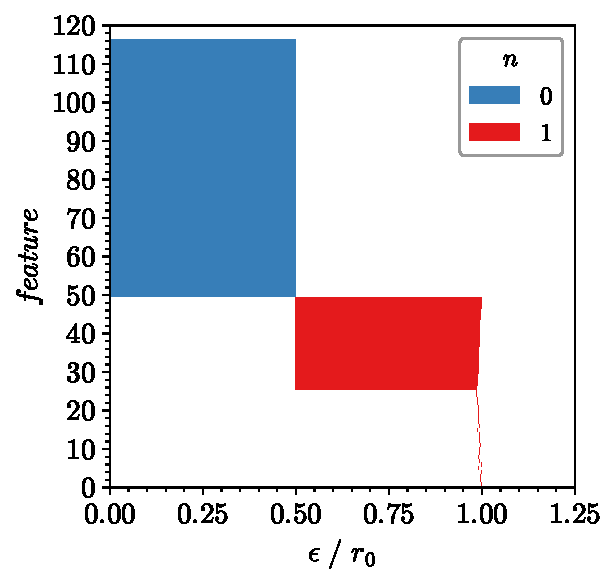
\includegraphics[width=\textwidth]{./figures/ph/ex_c_barcode.pdf}
         \caption{}
         \label{fig:exvisa}
     \end{subfigure}
     \hfill
     \begin{subfigure}[b]{0.45\textwidth}
         \centering
         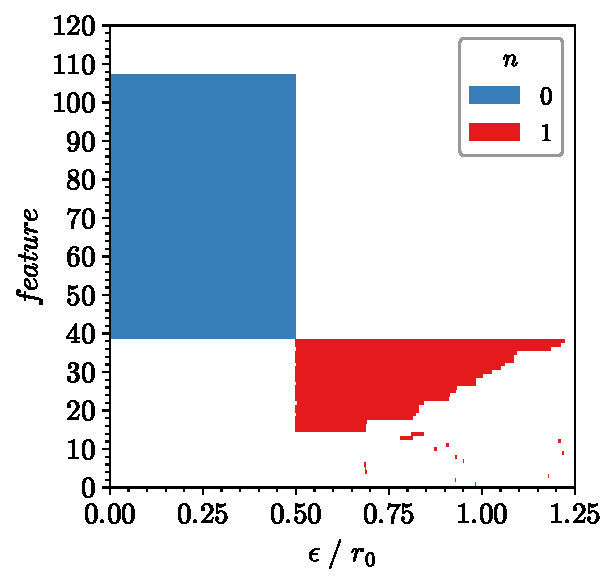
\includegraphics[width=\textwidth]{./figures/ph/ex_a_barcode.pdf}
         \caption{}
         \label{fig:exvisb}
     \end{subfigure}
     \hfill
     
     \begin{subfigure}[b]{0.45\textwidth}
         \centering
         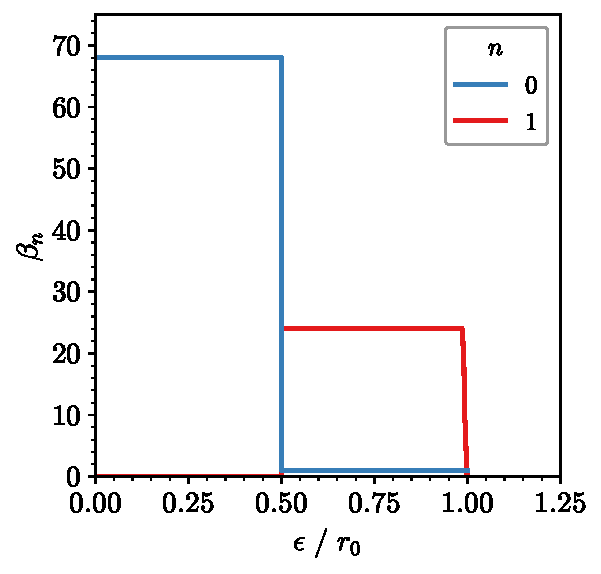
\includegraphics[width=\textwidth]{./figures/ph/ex_c_betti.pdf}
         \caption{}
         \label{fig:exvisc}
     \end{subfigure}
     \hfill
     \begin{subfigure}[b]{0.45\textwidth}
         \centering
         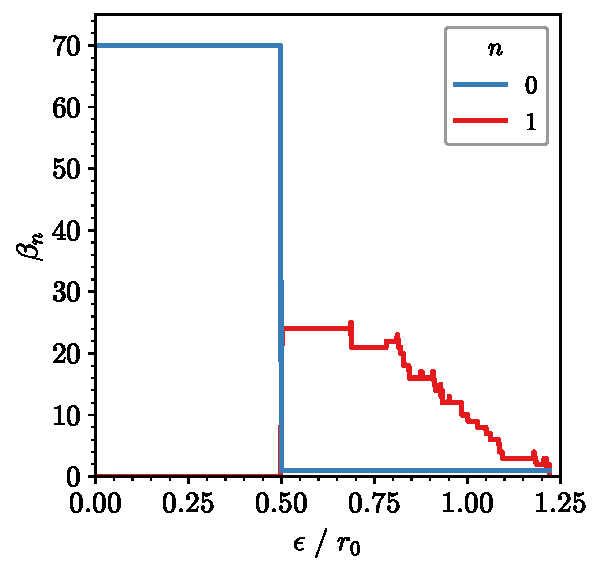
\includegraphics[width=\textwidth]{./figures/ph/ex_a_betti.pdf}
         \caption{}
         \label{fig:exvisd}
     \end{subfigure}
     \hfill
     
     \begin{subfigure}[b]{0.45\textwidth}
         \centering
         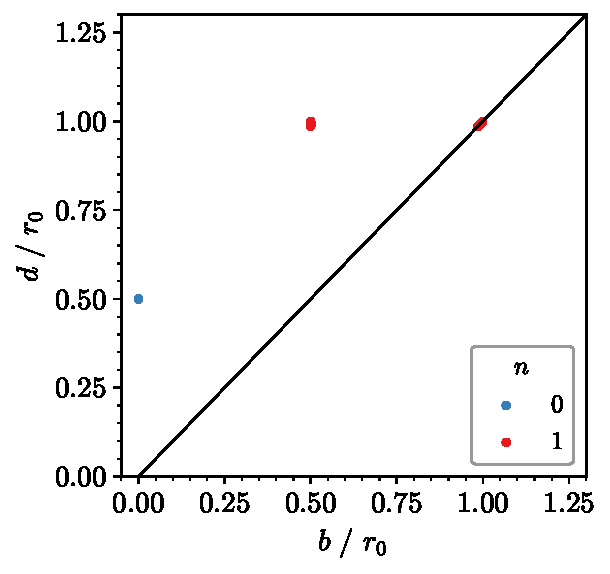
\includegraphics[width=\textwidth]{./figures/ph/ex_c_pd.pdf}
         \caption{}
         \label{fig:exvise}
     \end{subfigure}
     \hfill
     \begin{subfigure}[b]{0.45\textwidth}
         \centering
         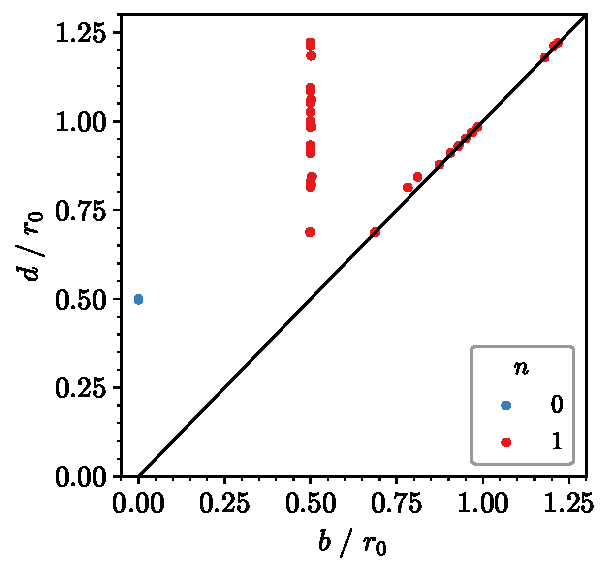
\includegraphics[width=\textwidth]{./figures/ph/ex_a_pd.pdf}
         \caption{}
         \label{fig:exvisf}
     \end{subfigure}
     \hfill
    
	\caption{Different methods for visualising results of persistence of topological features. The left column gives results for the example crystalline configuration in figure \ref{fig:phex}, and the right column the amorphous configuration in the same figure. Panels (a) and (b) show the persistence barcode, panels (c) and (d) the evolution in Betti numbers with filtration value and (e) and (f) the persistence diagram.}
	\label{fig:exvis}
\end{figure}

Although these visualisation methods have been introduced here, they will be interpreted only at a very high level, with more detailed analysis provided in the analysis sections.
Nevertheless, examining the results for the two example systems in \ref{fig:exvis}, one can see that the crystalline and amorphous systems have both similarities and differences.
To begin with, the 0\--dimensional features appear very similar across all plots, with $b=0$ and $d=r_0/2$.
This is because in atomic systems, the average bond length is highly restricted, and so all atoms become connected in a very small range of filtration values, corresponding to half the mean bond length (as the filtration value measures the circumradius of the 1\--simplex).
As such, the $0$\--dimensional features provide little insight for atomic systems, and will be neglected in the analysis in this chapter.

On the other hand, the 1\--dimensional features show significant differences between the crystalline and amorphous configurations.
Both systems have 24 persistent bars in their barcode (figures \ref{fig:exvisa} and \ref{fig:exvisb}), which are born at $\epsilon=r_0/2$, but the lifetimes vary considerably. 
For the crystalline system, all persistent cycles (corresponding to hexagons) terminate at almost the same value of $\epsilon=r_0$, whereas in the amorphous case there is a much broader distribution of values.
These values will be discussed in detail in section \ref{s:phbands}, but as might be expected, it is related to the radius of the circumcircle into which each polygon is inscribed. 
It is not only the persistent cycles which show variation though.
The persistence diagrams, figures \ref{fig:exvise} and \ref{fig:exvisf}, also show that the short lived features, which lie close to the line $b=d$, show greater variation in the amorphous case.
This will also be explored in greater depth in the remainder of the chapter.

What these small examples serve to demonstrate, is that persistent homology does show some promise for capturing the disorder in amorphous materials.
The question is whether these visualisations can be systematically interpreted to quantify this disorder, and obtain information which is not available via alternative methods.

\section{Persistent Homology with Triangle Rafts}

Persistent homology is first studied in reference to triangle rafts, introduced in chapter \ref{ch:bilayers}.
To briefly reiterate, triangle rafts are a model for \td{} amorphous silica, representing the bilayer of corner sharing tetrahedra as projected equilateral triangles.
Triangle rafts are characterised by having a diverse ring distributions, owing to the flexibility afforded to the structure by the oxygen linkages.
Coupled with this, the nearest\--neighbour Si\--Si distances remain in a relatively tight distribution, as shown in table \ref{tab:trsidist}, as a result of the rigidity imposed by the triangular subunits.

\begin{table}[hbt]
\centering
\caption{Relative nearest\--neighbour Si\--Si distances within different ring sizes in a triangle raft, assuming ring regularity.}
\label{tab:trsidist}
\begin{tabular}{cccccccc}
\toprule
$k$ & 4 & 5 & 6 & 7 & 8 & 9 & 10 \\
\midrule
Si\--Si & 0.966 & 0.995 & 1.000 & 0.997 & 0.991 & 0.985 & 0.978 \\
\bottomrule
\end{tabular}
\end{table}

An algorithm to construct triangle rafts was introduced in section \ref{s:triangleraft}.
The ring statistics in the resulting configurations can be tuned with a ``temperature'' parameter, $T$, with a higher temperature leading to the incorporation of more extreme ring sizes.
This is beneficial, as it allows a systematic evaluation of the results of persistent homology calculations, using configurations with a continuous evolution in structure.
As such, the samples from section \ref{s:triangleraft}, with ring sizes in the range $k=4\rightarrow10$, were analysed using the GUDHI library \cite{gudhi}.
In these analyses, only the silicon positions were included, as the oxygen positions are in a sense ``degenerate'' (as they do not affect the ring topologies) and would only serve to obscure the calculation.
In addition, this makes the cycles computed by persistent homology consistent with the definitions of rings elsewhere in this thesis.

The results of the persistent homology calculations will be discussed primarily in terms of the persistence diagrams, with the structure rationalised in comparison to analytic examples. 
However, it will also be shown how metrical quantities such as the ring statistics compare to inferred persistent cycles.

\subsection{Overview of Persistence Diagrams}

The persistence diagrams for triangle rafts at four increasing temperatures are shown in figures \ref{fig:trpda}\--\ref{fig:trpdd}, combined across multiple configurations.
Discussing first the overall structure, one can see there is a definite systematic evolution in behaviour as temperature (and therefore disorder) increases.
To aid discussion, points will be referred to in terms of birth\--death pairs, $\left(b,d\right)$, with filtration values given in reference to the equilibrium bond length, $r_0$.

At the lowest temperature, configurations are dominated largely by regular hexagons with few defects, reflected in the persistence diagram by bright spots at $\bd{0.5}{1.0}$ and $\bd{1.0}{1.0}$ (in comparison with figure \ref{fig:exvise}).
As the temperature increases, and rings of different sizes are introduced, characteristic bands form in the persistence diagram, which are most intense at low lifetimes (\ie{} close to $b=d$) and then ``wash out'' at lower birth values and longer lifetimes. 
At higher temperatures still, these bands broaden and finally coalesce.

\begin{figure}[tb]
	\centering
     
      \begin{subfigure}[b]{0.48\textwidth}
         \centering
         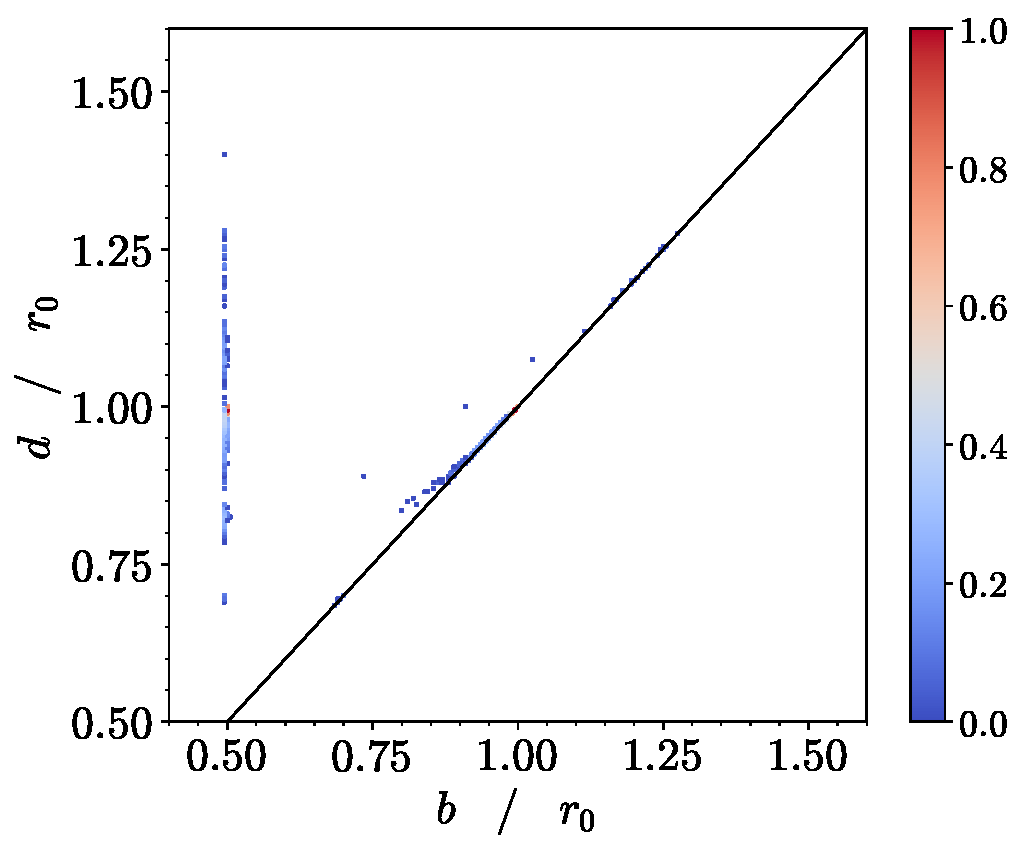
\includegraphics[width=\textwidth]{./figures/ph/t-4500_tr_pd.pdf}
         \caption{$T=10^{-4.5}$, $p_6=0.997$}
         \label{fig:trpda}
     \end{subfigure}
     \hfill
      \begin{subfigure}[b]{0.48\textwidth}
         \centering
         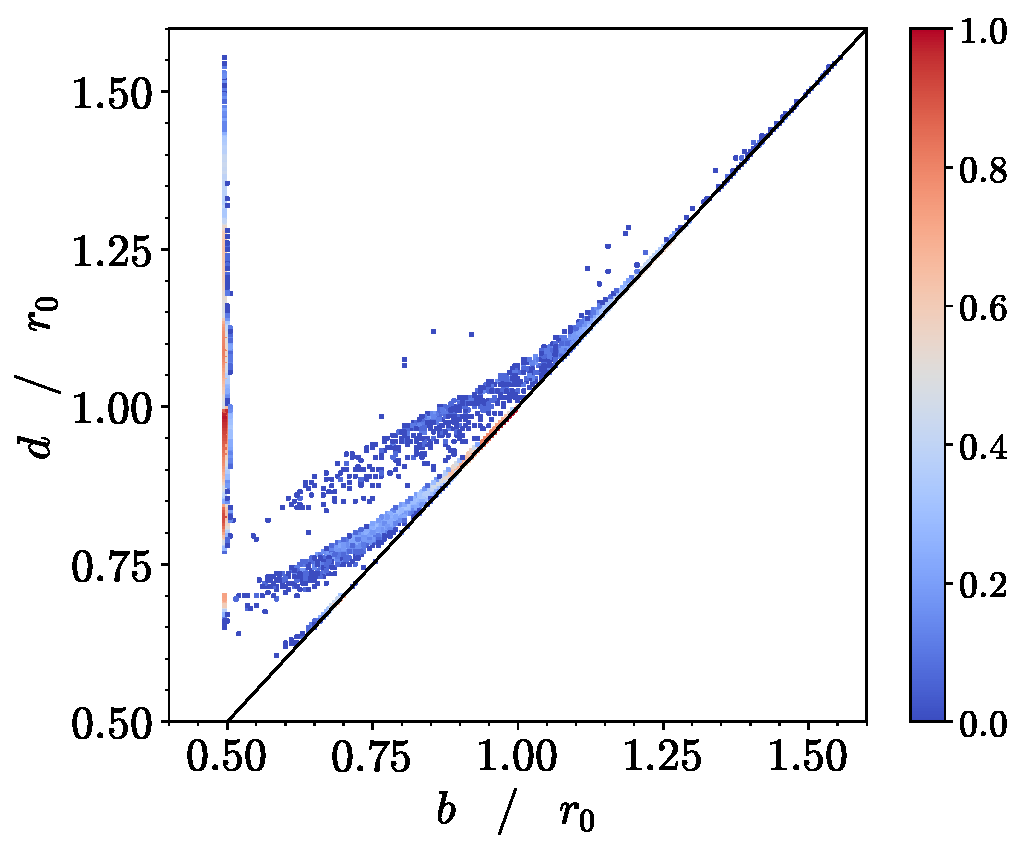
\includegraphics[width=\textwidth]{./figures/ph/t-3600_tr_pd.pdf}
         \caption{$T=10^{-3.6}$, $p_6=0.668$}
         \label{fig:trpdb}
     \end{subfigure}
     \hfill
     	
     \vspace{2mm}
     \begin{subfigure}[b]{0.48\textwidth}
         \centering
         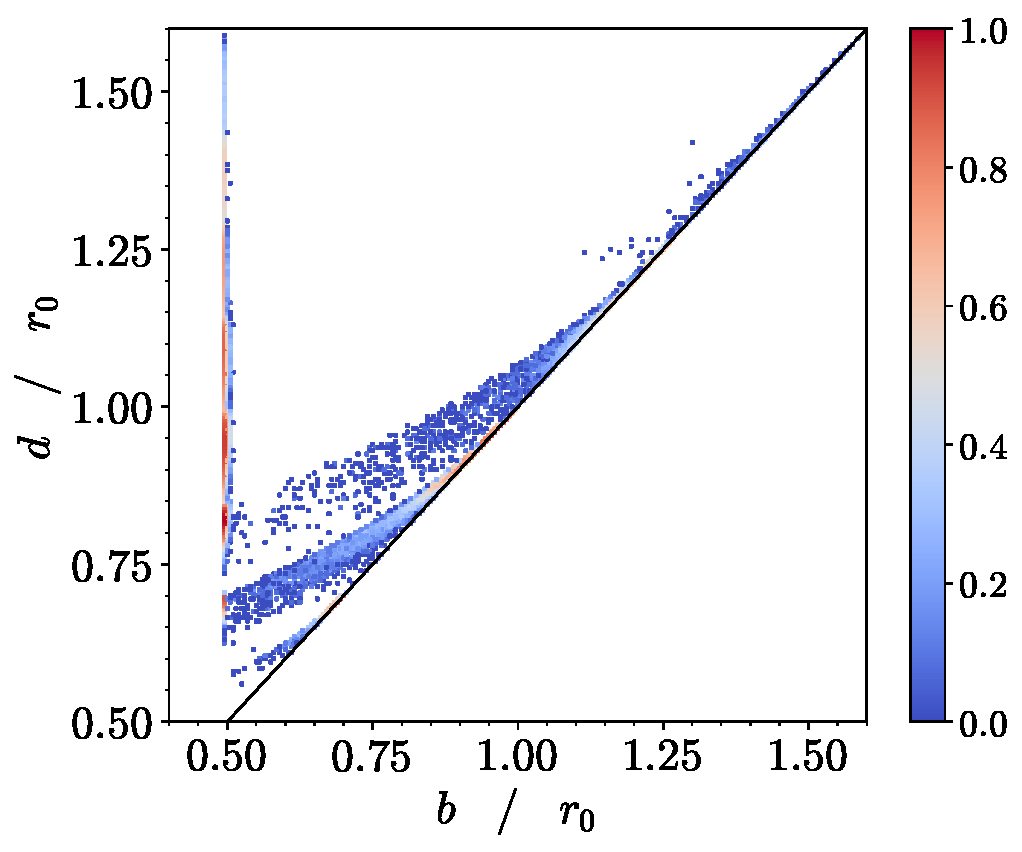
\includegraphics[width=\textwidth]{./figures/ph/t-2700_tr_pd.pdf}
         \caption{$T=10^{-2.7}$, $p_6=0.354$}
         \label{fig:trpdc}
     \end{subfigure}
     \hfill
      \begin{subfigure}[b]{0.48\textwidth}
         \centering
         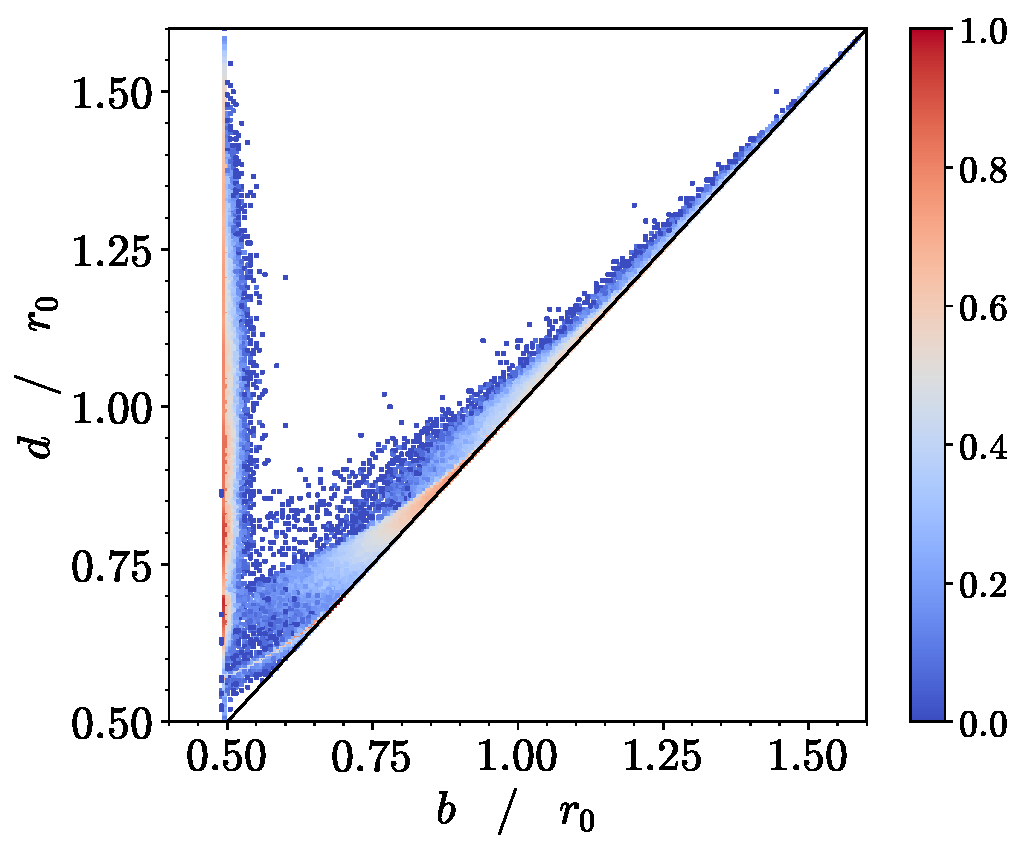
\includegraphics[width=\textwidth]{./figures/ph/t-1800_tr_pd.pdf}
         \caption{$T=10^{-1.8}$, $p_6=0.211$}
         \label{fig:trpdd}
     \end{subfigure}
     \hfill
    
	\caption{Persistence diagrams for triangle rafts generated at increasing temperatures and disorder (as indicated in captions). Points are coloured by multiplicity to highlight structure. The line $b=d$ is also indicated as a diagonal black line.}
	\label{fig:trpd}
\end{figure}

This band structure and its associated behaviour has been observed before in studies of three\--dimensional amorphous silica \cite{Nakamura2015,Hiraoka2016,Robins2017}.
These papers often identify spots in the bands which correspond to known structures, and Hiraoka \etal{} go as far as suggesting that the bands correspond to rings formed from different nearest\--neighbour length scales \cite{Hiraoka2016}.
However, this was proposed by observing the cycles directly, and the interpretation is somewhat more complicated by the inclusion of oxygen atoms.
By studying this problem in two dimensions, it can now be shown that these bands arise from the formation of rings between nearest\--neighbour, second nearest\--neighbour, and successively higher order interactions.


\subsection{Band Structure in Persistence Diagrams}
\label{s:phbands}

Before rationalising the band structure observed in the persistence diagrams of triangle rafts, it is useful to consider again the process of cycle formation in persistent homology.
The important points are summarised below:
\begin{enumerate}
	\item A cycle is born when a 1\--simplex cuts a previous cycle in two. The birth value of the new cycle is then equal to the filtration value of the 1\--simplex.
	\item A cycle dies dies when \textit{all} of the 2\--simplices within it are present. The death value is then equal to the highest filtration value of the  constituent 2\--simplices.
	\item A cycle is only counted if the death value is strictly greater than the birth value.
	\item As a result of the above, a cycle will only persist if the 1\--simplex which creates it has a lower filtration value than the 2\--simplex which destroys it.
\end{enumerate}
Understanding these properties is key to interpreting the results of persistence diagrams.

To explore the origins of the band structure, an ideal set of polygons will primarily be considered, where all sides have unit length.
As previously mentioned, this approximation is reasonable for triangle rafts.
The first, and simplest, band to consider is the vertical band at $b=0.5r_0$, which displays bright spots along its length.
These correspond to the cycles initially formed when 1\--simplices connect adjacent atoms, which have a circumradius of half the edge length.
This band therefore originates from cycles pertaining to the nearest\--neighbour interactions, and so will be referred to as the band $B_1$.
These cycles will only die when all the 2\--simplices inside them are present.
As an illustration, a model is introduced whereby cycles are treated as a regular polygon with unit side lengths.
By definition, in this case all simplices must have the same filtration value, as they lie on a common circle (see for example figure \ref{fig:b3b}).
The filtration values for these simplices are given by:
\begin{equation}
	\Phi_k = \frac{1}{2\sin\left(\pi/k\right)}\,,
\end{equation}
where $\Phi_k$ will be used to denote the circumradius in a regular $k$\--sided polygon with unit edge lengths.
The values of $\Phi_k$ for $4\leq k \leq 10$ can be found in table \ref{tab:circumradii}.
It follows that a regular polygon will have a death value at $\Phi_k$, and furthermore, no more cycles will be born out of this point set.
Although difficult to see, these values of $\Phi_k$ correspond well with the bright spots in the persistence diagrams in figure \ref{fig:trpd}, as will become more apparent in subsequent analyses in this chapter.

\begin{figure}[tb]
	\centering
     
      \begin{subfigure}[b]{0.45\textwidth}
         \centering
         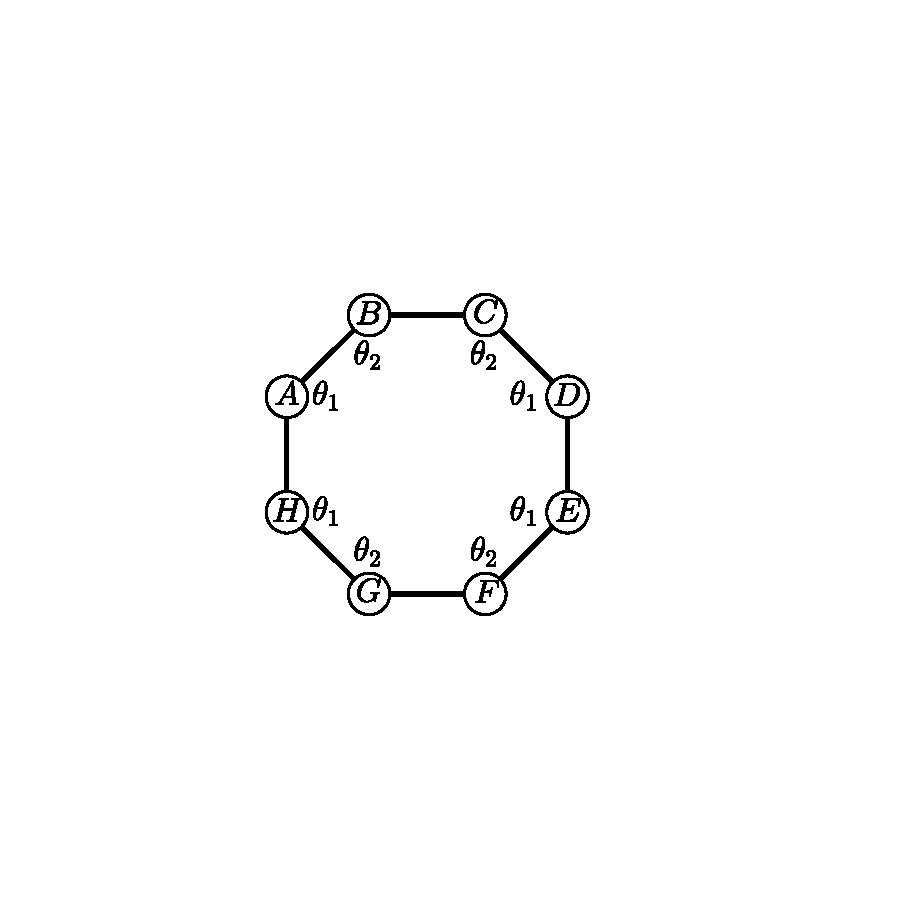
\includegraphics[width=0.45\textwidth]{./figures/ph/sl_oct_b3_135x.pdf}
         \caption{\phantom{xxx} \\ \phantom{xxx}}
         \label{fig:b3a}
     \end{subfigure}
     \hfill
     \begin{subfigure}[b]{0.45\textwidth}
         \centering
         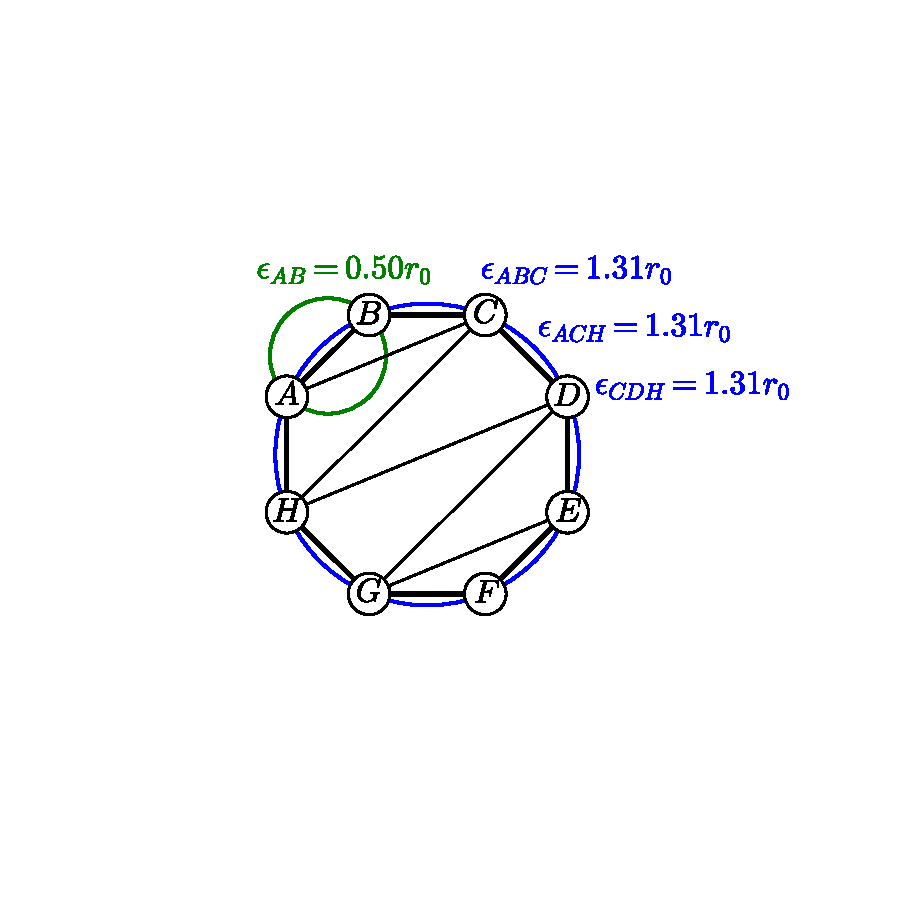
\includegraphics[width=0.7\textwidth]{./figures/ph/sl_oct_b3_135.pdf}
         \caption{$\theta_1=135^\circ$; \\$\left(0.50,1.31\right)$}
         \label{fig:b3b}
     \end{subfigure}
     
     \vspace{2mm}
   \begin{subfigure}[b]{0.32\textwidth}
         \centering
         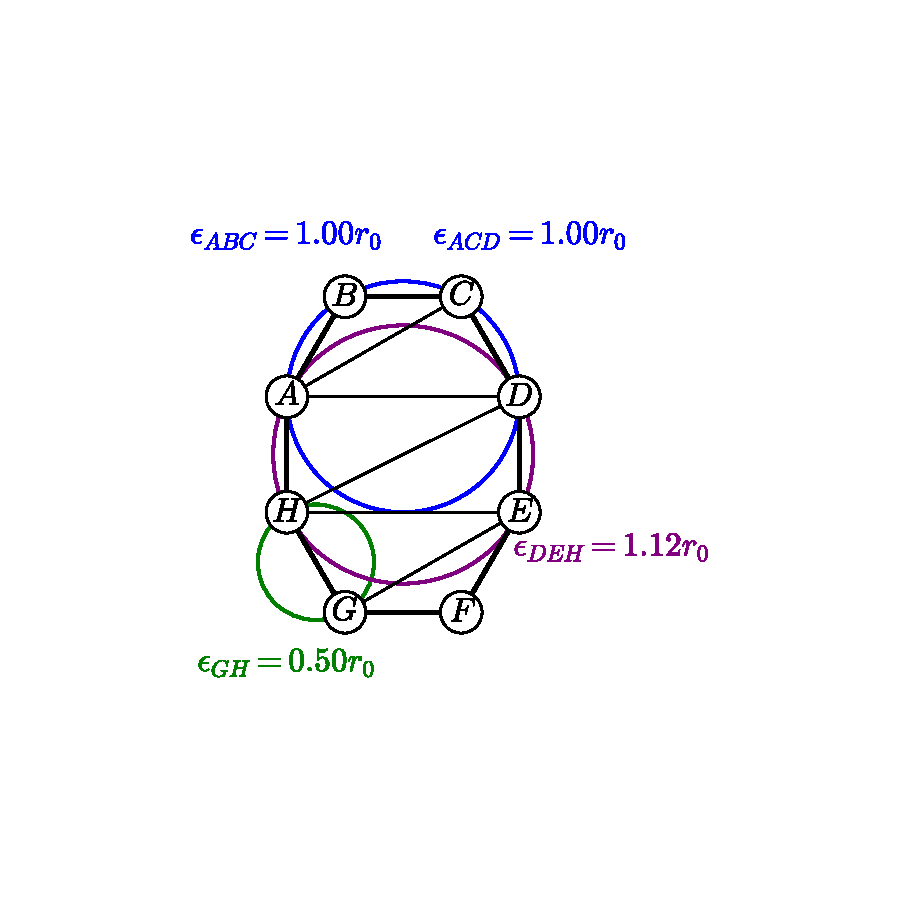
\includegraphics[width=\textwidth]{./figures/ph/sl_oct_b3_150.pdf}
         \caption{$\theta_1=150^\circ$; \\$\left(0.50,1.12\right)$}
         \label{fig:b3c}
     \end{subfigure}
     \hfill
     \begin{subfigure}[b]{0.32\textwidth}
         \centering
         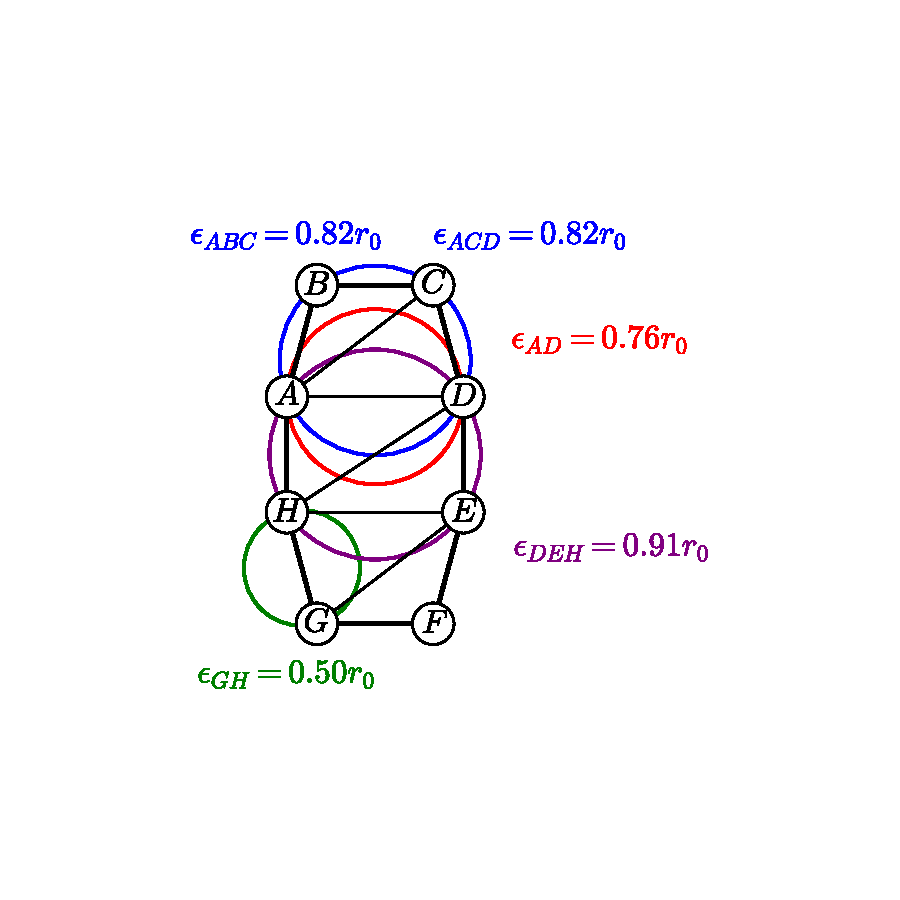
\includegraphics[width=\textwidth]{./figures/ph/sl_oct_b3_165.pdf}
         \caption{$\theta_1=165^\circ$; \\$\left(0.50,0.91\right)$, $\left(0.76,0.82\right)$ }
         \label{fig:b3d}
     \end{subfigure}
      \hfill
     \begin{subfigure}[b]{0.32\textwidth}
         \centering
         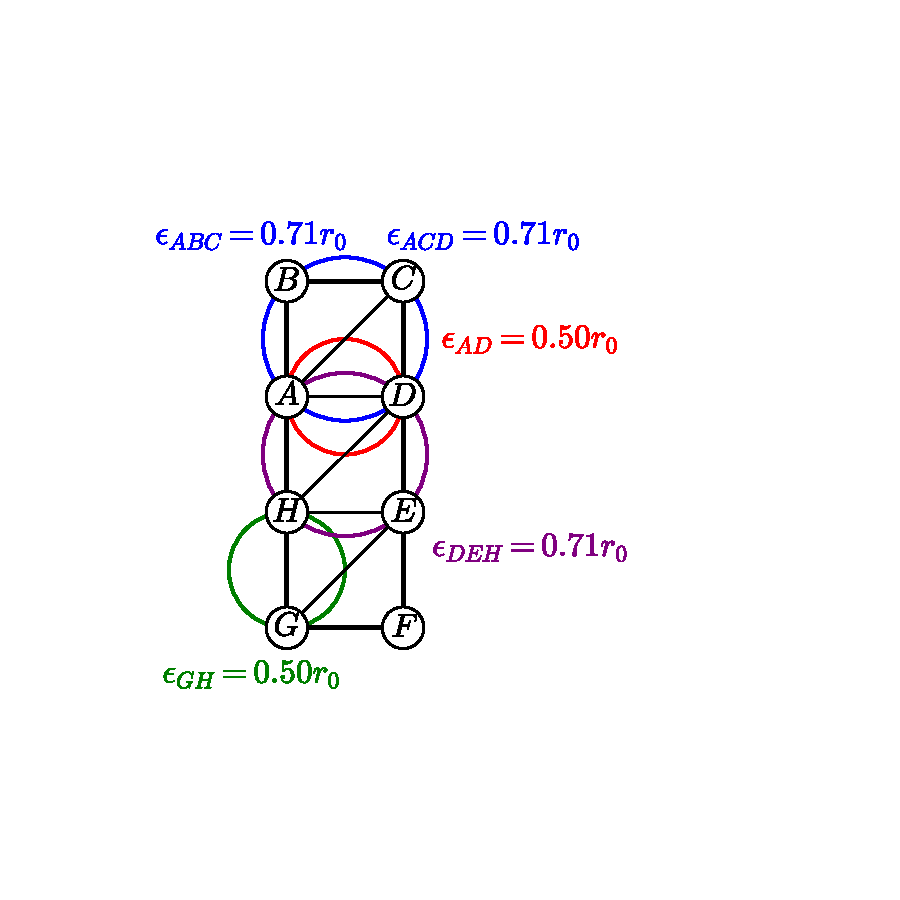
\includegraphics[width=0.9\textwidth]{./figures/ph/sl_oct_b3_180.pdf}
         \caption{$\theta_1=180^\circ$; \\$\left(0.50,0.71\right)$}
         \label{fig:b3e}
     \end{subfigure}
   
	\caption{Systematic distortions of an octagon with unit side lengths, and the effect on the corresponding persistent cycles. Panel (a) shows the octagon model, which is defined in terms of two angles. Panels (b)\--(e) show a series of distortions. For each panel the angles and persistence $\bd{b}{d}$ pairs are given in the caption. In addition, the circumcircles of selected simplices are highlighted, with the corresponding filtration values colour coded. The Delaunay triangulation is given as the interior black lines. These diagrams outline the origin of the $B_1$ and $B_3$ bands.}
	\label{fig:b3}
\end{figure}

\begin{table}[hbt]
\centering
\caption{Circumradii of regular polygons with unit edge lengths.}
\label{tab:circumradii}
\begin{tabular}{cccccccc}
\toprule
$k$ & 4 & 5 & 6 & 7 & 8 & 9 & 10 \\
\midrule
$\Phi_k$ & 0.707 & 0.851 & 1.000 & 1.152 & 1.307 & 1.462 & 1.618 \\
\bottomrule
\end{tabular}
\end{table}

However, the vertical band clearly shows a continuum of values, not discrete points.
Therefore, a modification to the model can be considered, whereby all edge lengths are maintained at unity, but the polygon undergoes a systematic distortion - begin compressed about an axis passing through two opposite edges.
This process is highlighted in figures \ref{fig:b3a}\--\ref{fig:b3e}.
In this part of the analysis, only the persistence cycles which are born at $b=0.5r_0$ are of interest.
These cycles will die when the Delaunay triangulation is realised.
This is achieved when the simplex with the highest filtration value, here $DEH$ or $ADH$, is present.
As the polygon is compressed, it can be seen that the circumcircle for this simplex (purple circle) is reduced.
In other words, distortion of the polygon acts to reduce the lifetime of the original cycle born at $b=0.5r_0$.
The consequence of this is that the band $B_1$ manifests, instead of a simple series of discrete points.

The distortions in figures \ref{fig:b3a}\--\ref{fig:b3e} demonstrate the phenomenon central to the discussion of the remaining bands: that between some critical values of $\theta$, a second cycle is born within the first.
This is only possible when the 1\--simplex $AD$ has a filtration value less than the 2\--simplex $ACD$.
In figure \ref{fig:b3c} where $\theta_1=150^\circ$, this is \textit{not} the case, as $AD$ and $ACD$ share the same filtration value.
This is in fact the limiting case, and beyond this angle the circumcircle for $AD$ (red circle) is not contained within that for $ACD$ (blue circle), it has a smaller radius, and therefore filtration value.
The persistence of this cycle will therefore range between $\bd{0.5}{0.71}$, $\bd{0.76}{0.82}$ and $\bd{1.0}{1.0}$.
The intermediate values can be found via numerically scanning the angle range, but even from these points it is clear that this corresponds well with the most prominent ``central'' band in the persistence diagram.
Furthermore, this band arises from the cycles formed by connecting neighbours three bonds apart.
Although shown for the octagon here, this in fact holds for the other ring sizes that can support this (\ie{} $k>5$), and so this band is termed $B_3$.

\begin{figure}[tbp]
	\centering
     
      \begin{subfigure}[b]{0.45\textwidth}
         \centering
         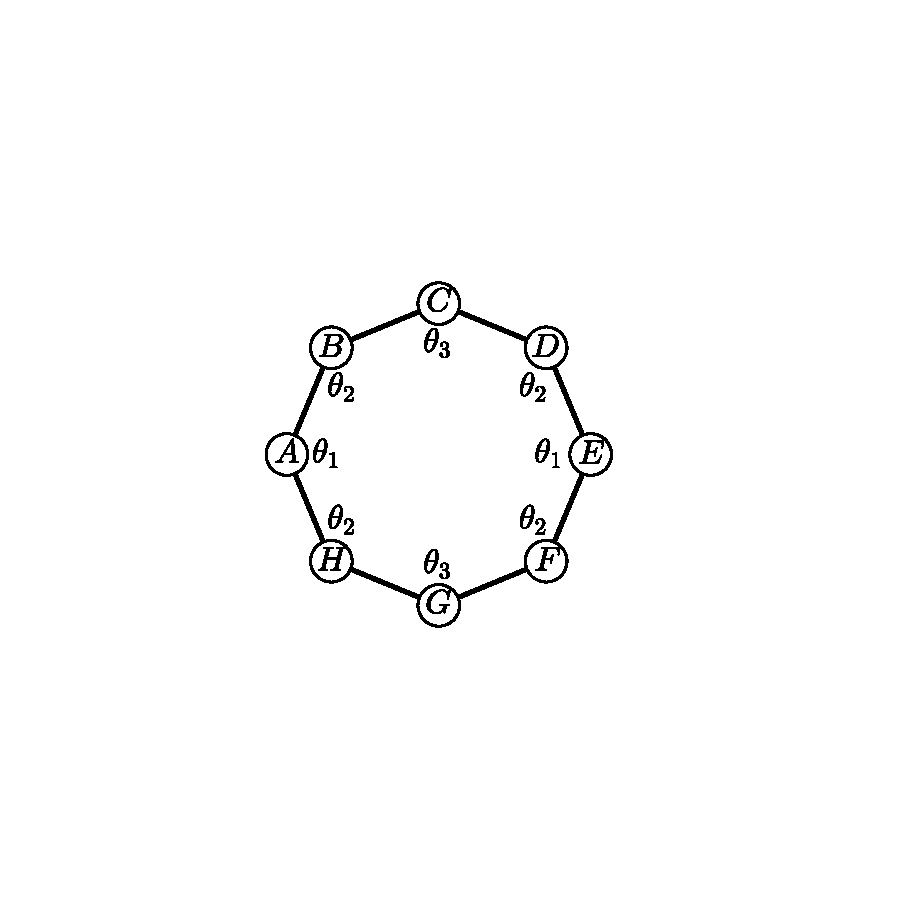
\includegraphics[width=0.45\textwidth]{./figures/ph/sl_oct_b4_135x.pdf}
         \caption{\phantom{xxx} \\ \phantom{xxx}}
         \label{fig:b4a}
     \end{subfigure}
     \hfill
     \begin{subfigure}[b]{0.45\textwidth}
         \centering
         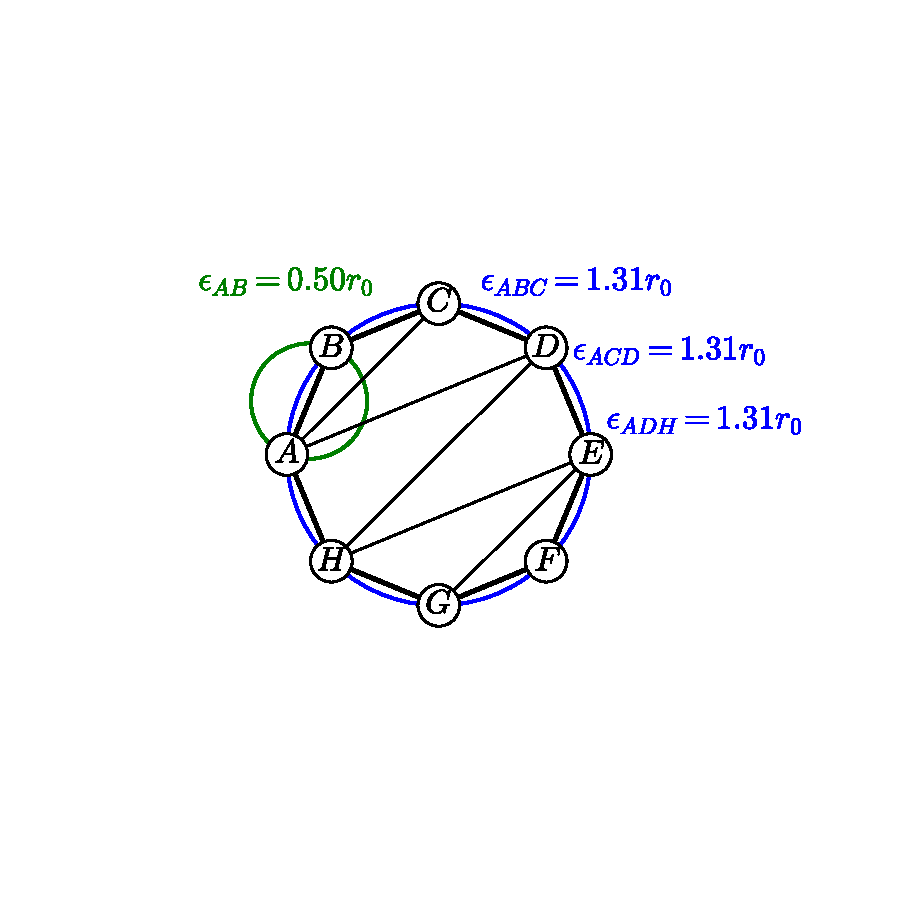
\includegraphics[width=0.8\textwidth]{./figures/ph/sl_oct_b4_135.pdf}
         \caption{$\theta_1=135^\circ$, $\theta_2=135^\circ$; \\$\left(0.50,1.31\right)$}
         \label{fig:b4b}
     \end{subfigure}
     
     \vspace{2mm}
   \begin{subfigure}[b]{0.32\textwidth}
         \centering
         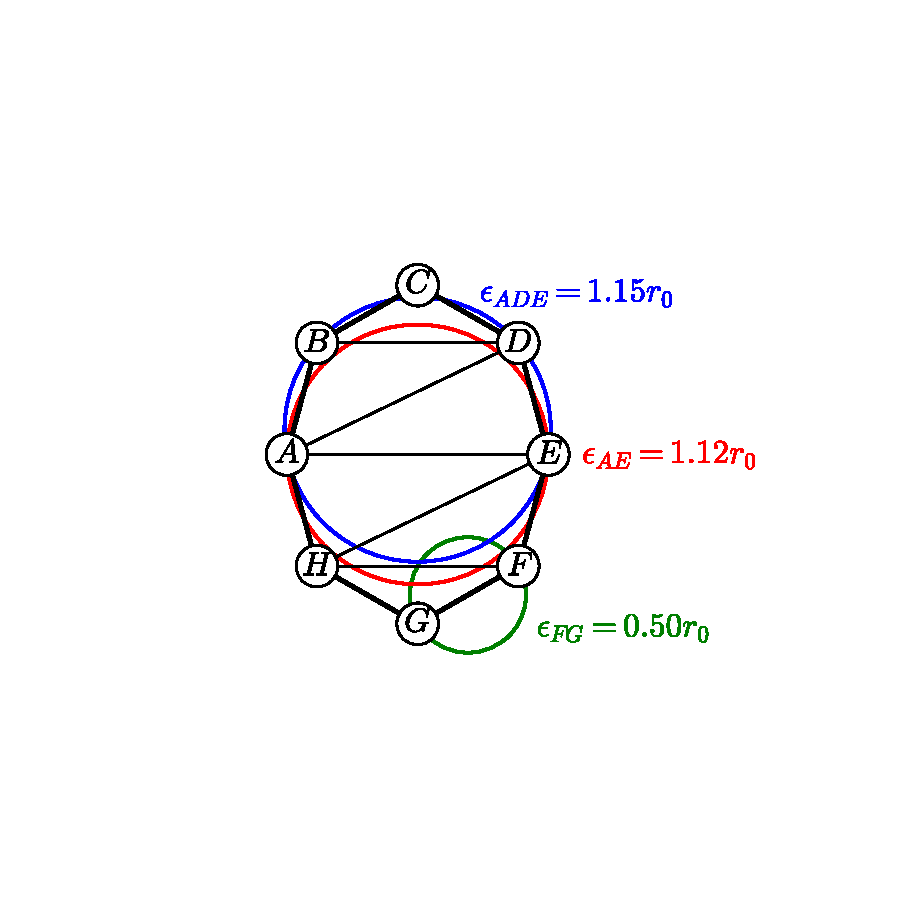
\includegraphics[width=0.95\textwidth]{./figures/ph/sl_oct_b4_150.pdf}
         \caption{$\theta_1=150^\circ$, $\theta_2=135^\circ$; \\$\left(0.50,1.15\right)$, $\left(1.12,1.15\right)$}
         \label{fig:b4c}
     \end{subfigure}
     \hfill
     \begin{subfigure}[b]{0.32\textwidth}
         \centering
         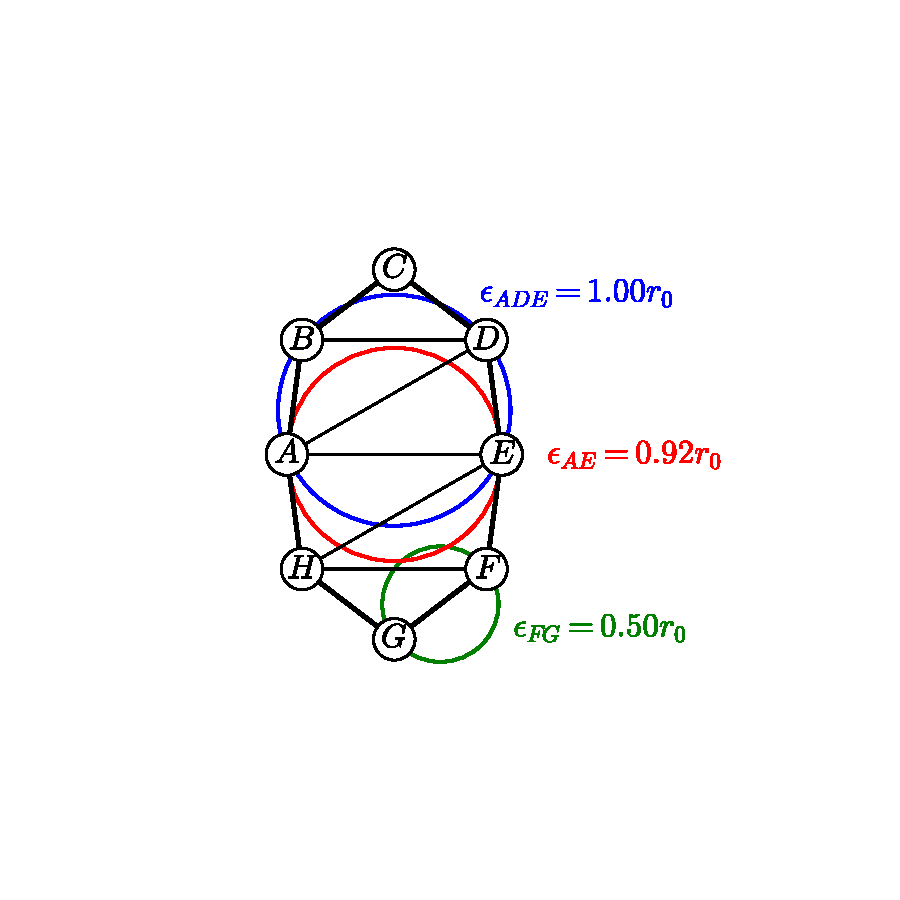
\includegraphics[width=0.85\textwidth]{./figures/ph/sl_oct_b4_165.pdf}
         \caption{$\theta_1=165^\circ$, $\theta_2=135^\circ$; \\$\left(0.50,1.00\right)$, $\left(0.92,1.00\right)$}
         \label{fig:b4d}
     \end{subfigure}
      \hfill
     \begin{subfigure}[b]{0.32\textwidth}
         \centering
         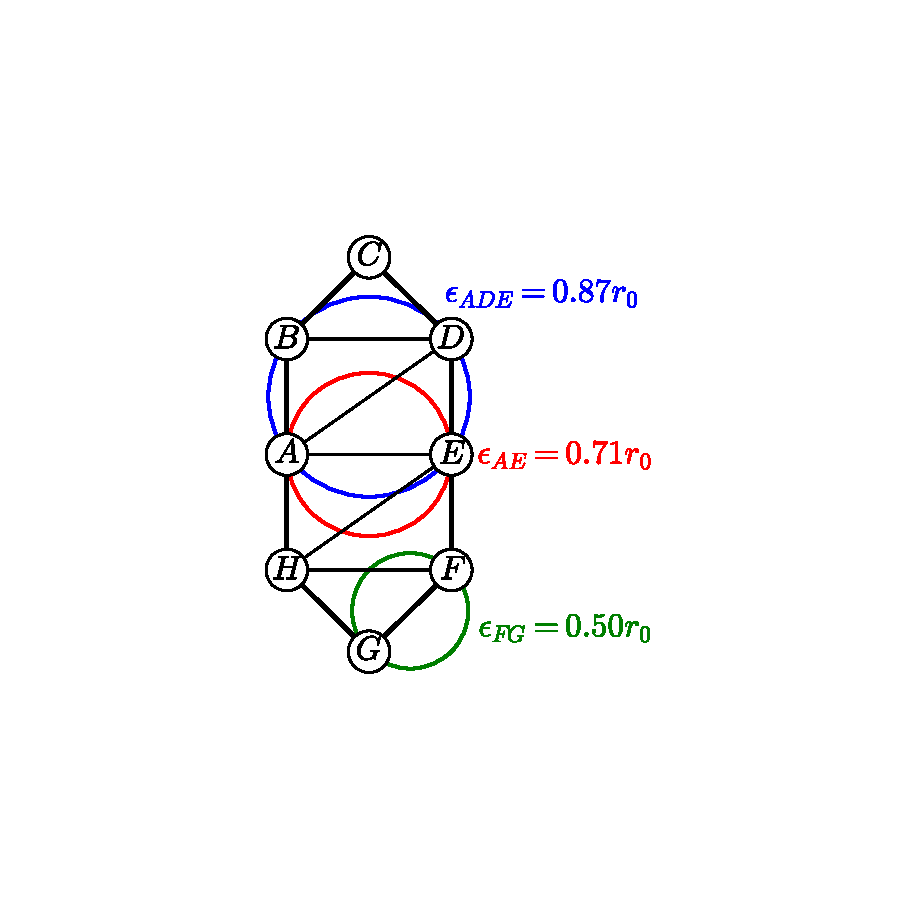
\includegraphics[width=0.75\textwidth]{./figures/ph/sl_oct_b4_180.pdf}
         \caption{$\theta_1=180^\circ$, $\theta_2=135^\circ$; \\$\left(0.50,0.87\right)$, $\left(0.71,0.87\right)$}
         \label{fig:b4e}
     \end{subfigure}
   
   \vspace{2mm}
   \begin{subfigure}[b]{0.32\textwidth}
         \centering
         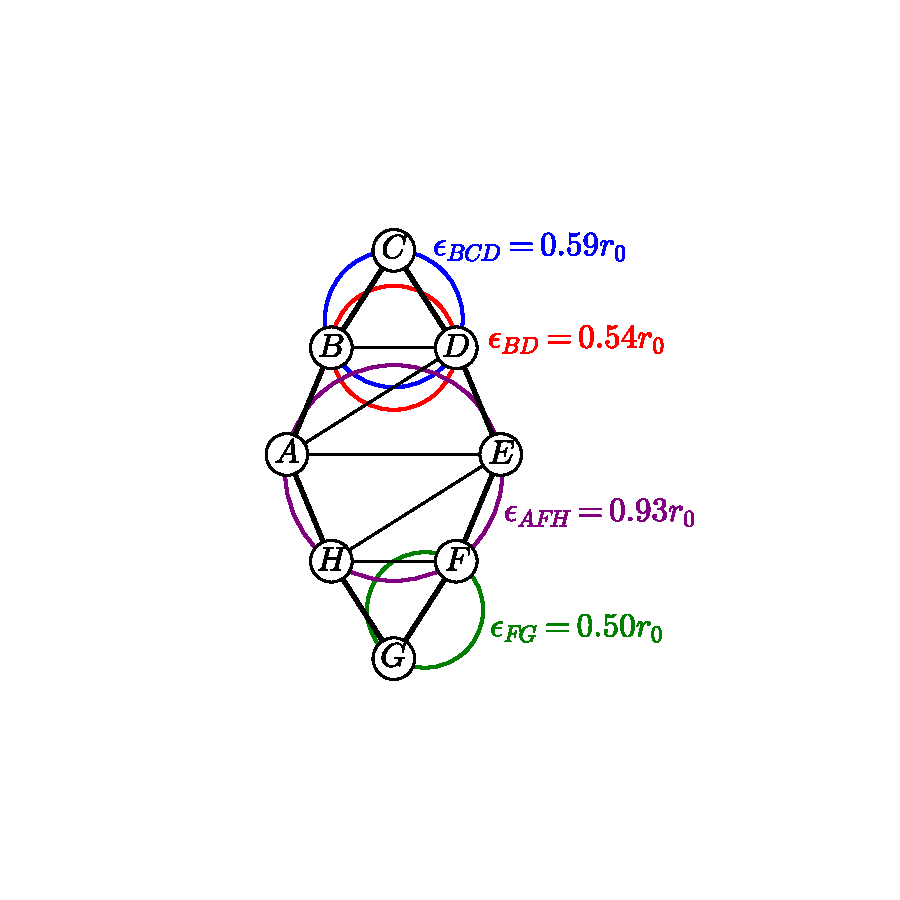
\includegraphics[width=0.8\textwidth]{./figures/ph/sl_oct_b2_a.pdf}
         \caption{$\theta_1=135^\circ$, $\theta_2=170^\circ$; \\$\left(0.50,0.93\right)$, $\left(0.54,0.59\right)$}
         \label{fig:b4f}
     \end{subfigure}
     \hfill
     \begin{subfigure}[b]{0.32\textwidth}
         \centering
         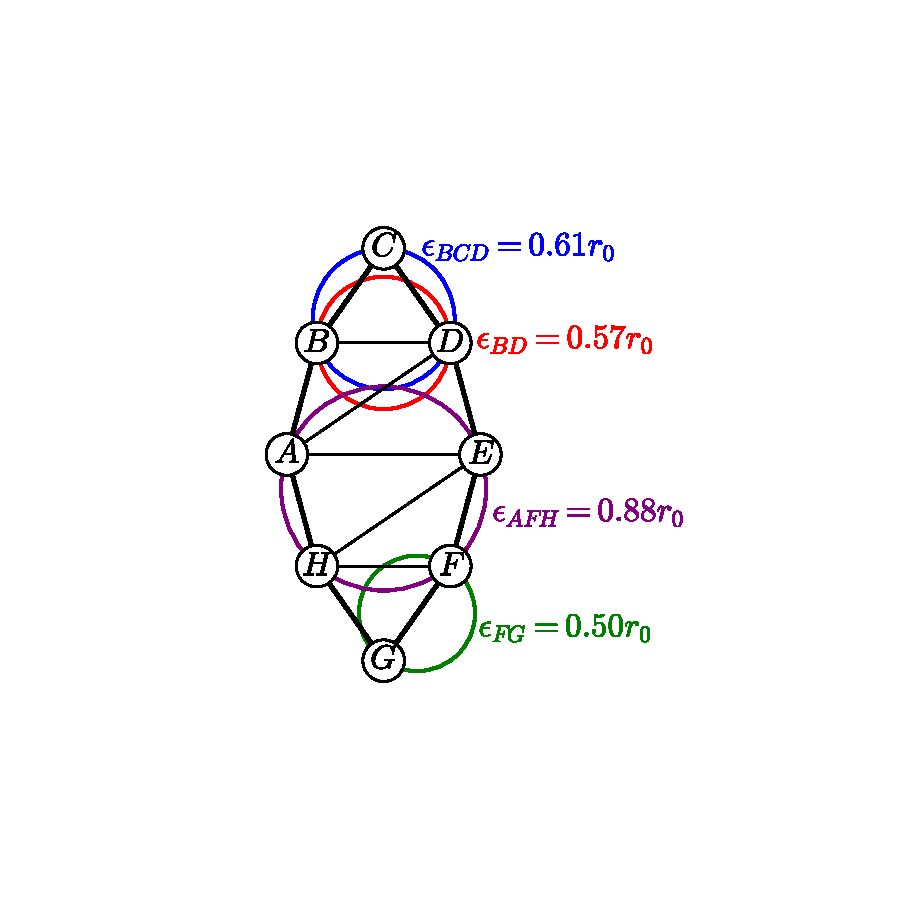
\includegraphics[width=0.8\textwidth]{./figures/ph/sl_oct_b2_b.pdf}
         \caption{$\theta_1=150^\circ$, $\theta_2=160^\circ$; \\$\left(0.50,0.88\right)$, $\left(0.57,0.61\right)$}
         \label{fig:b4g}
     \end{subfigure}
      \hfill
     \begin{subfigure}[b]{0.32\textwidth}
         \centering
         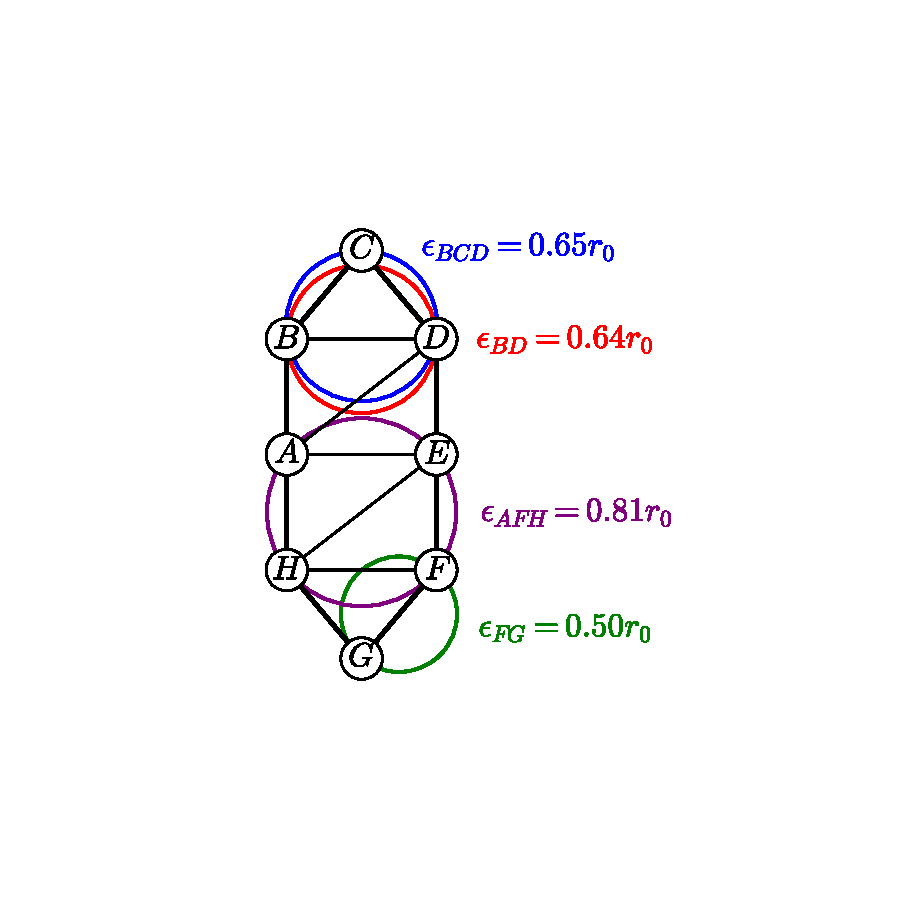
\includegraphics[width=0.8\textwidth]{./figures/ph/sl_oct_b2_c.pdf}
         \caption{$\theta_1=180^\circ$, $\theta_2=140^\circ$; \\$\left(0.50,0.81\right)$, $\left(0.64,0.65\right)$}
         \label{fig:b4h}
     \end{subfigure}

	\caption{Further systematic distortions of an octagon with unit side lengths, and the effect on the corresponding persistent cycles. Panel (a) shows the octagon model, which is defined in terms of three angles. Panels (b)\--(h) show a series of distortions. For each panel the angles and persistence $\bd{b}{d}$ pairs are given in the caption (for panels (f)\--(h) an additional cycle is present, contributing to $B_3$, which is omitted for simplicity). In addition, the circumcircles of selected simplices are highlighted, with the corresponding filtration values colour coded. The Delaunay triangulation is given as the interior black lines. These diagrams outline the origin of the $B_2$ and $B_4$ bands.}
	\label{fig:b4}
\end{figure}

It might now be clear that the other bands can also be related to specific nearest\--neighbour interactions.
In order to demonstrate this, again the octagonal case can be examined, but with different ring distortions.
Now compression is about an axis through two opposite vertices, outlined in figure \ref{fig:b4}.
Figures \ref{fig:b4c}\--\ref{fig:b4e} illustrate how secondary cycle can be born at relatively high filtration values.
Here compression causes the 1\--simplex $AE$ to have a filtration value lower than the 2\--simplex $ADE$, enabling formation of a second cycle.
The atoms $A,E$ are separated by four bonds and so the corresponding band for such species is $B_4$.
The as\--yet unaccounted for band, at the lowest persistence, naturally must be $B_2$, arising from atoms separated by two bonds.
Examples of the formation of $B_2$ in the octagon are given in figures \ref{fig:b4f}\--\ref{fig:b4h}, corresponding to a ``pinch''.

For the octagon it is relatively difficult to add to the $B_2$ band.
This is worth some consideration. 
It has been stated that this analysis is not unique to the octagon, which has merely been selected for illustrative purposes as it \textit{can} display all the required behaviour.
However, in general large polygons ($k>6$) require little distortion to yield $B_3$ and $B_4$ bands, whereas significant rearrangement would be needed to contribute to $B_2$.
On the other hand, the $B_2$ band readily forms for small polygons $k<6$ and indeed the higher bands are inaccessible.
The most common polygon, the hexagon, most easily forms secondary cycles in $B_3$, and to a lesser extend $B_2$. 
This explains the relative prominence of this central $B_3$ band in figures \ref{fig:trpda}\--\ref{fig:trpdd}.
Furthermore, it is equally possible to obtain higher bands still, with sufficiently large polygons.
In the case of the triangle rafts in this section, the decagon in fact leads to the presence of a weak $B_5$ band.

\begin{figure}[tb]
	\centering
     
     \begin{subfigure}[b]{0.48\textwidth}
         \centering
         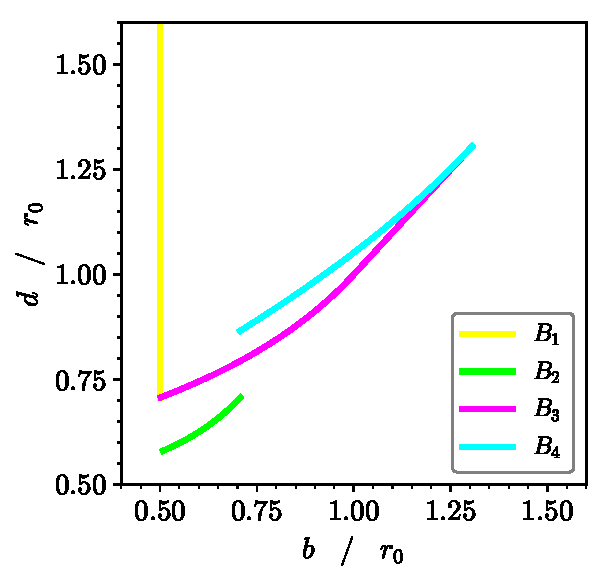
\includegraphics[width=0.88\textwidth]{./figures/ph/blines.pdf}
         \caption{}
         \label{fig:blinesa}
     \end{subfigure}
     \hfill
      \begin{subfigure}[b]{0.48\textwidth}
         \centering
         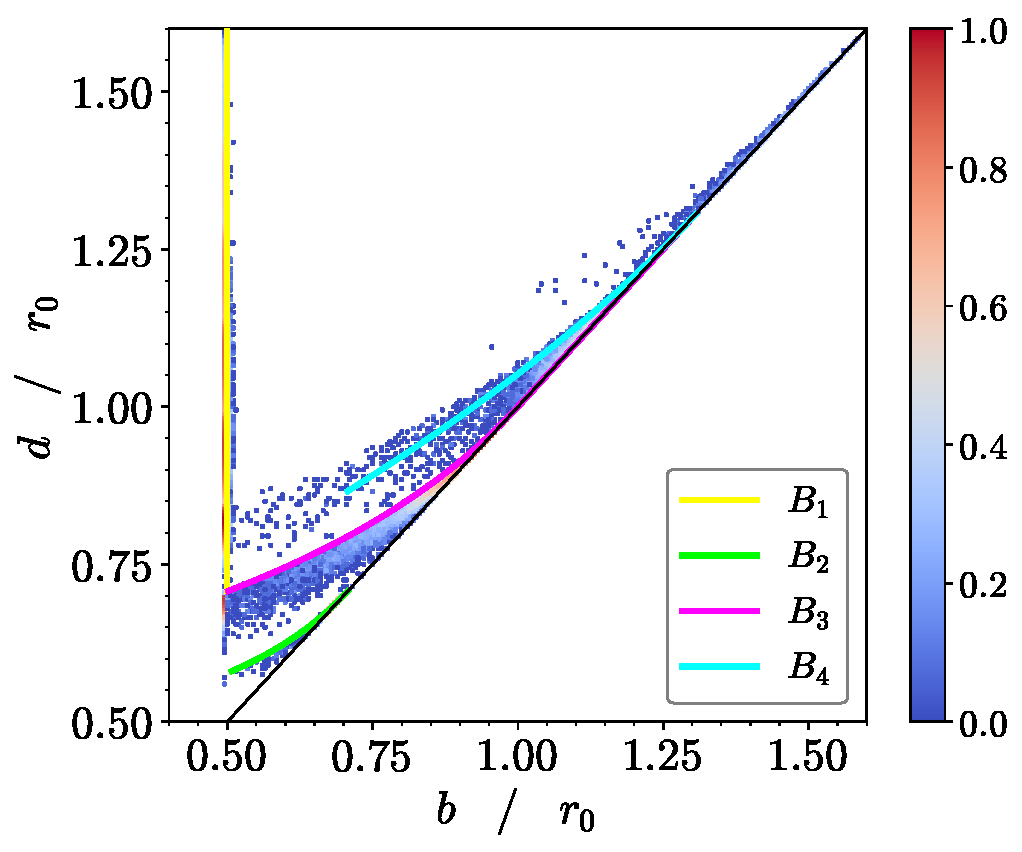
\includegraphics[width=\textwidth]{./figures/ph/blines_overlay.pdf}
         \caption{}
         \label{fig:blinesb}
     \end{subfigure}
 
	\caption{Bands corresponding to different nearest\--neighbour interactions, as calculated numerically using idealised models. Panel (a) shows the isolated lines, whilst panel (b) overlays them on the persistence diagram for triangle rafts from figure \ref{fig:trpdc}, to which there is good agreement}.
	\label{fig:blines}
\end{figure}

To conclude this section, the reasoning outlined above is tested by generating the bands numerically (distorting polygons conforming to the various idealised models), and comparing to the persistence diagrams of triangle rafts. 
The results are given in figure \ref{fig:blines}, which are quite compelling.
The shapes and positions of the various bands match well with those in the persistence diagrams from triangle rafts.
Furthermore, the intensities agree with the previous discussion, with the $B_3$ band being by far the most prominent.
It should be noted that the $B_3$ band calculated from the idealised model corresponds to the upper limit of that found from triangle raft simulations.
This is also as expected, as distortions in bond lengths and will only serve to reduce the death value. 
This is because, as table \ref{tab:trsidist} shows, the nature of the triangle raft model (of hinged near\--rigid triangles), means that the bond lengths can only be less than the equilibrium value, which leads to a concomitant decrease in the circumradii.
Overall, the relative simplicity and rigidity of the triangle raft model has enabled the structure of persistence diagrams to be well understood in this \td{} case.

\subsection{Cycles, Betti Numbers and Ring Statistics}

In addition to the persistence diagrams, information is also available through the first Betti number, $\beta_1$, which quantifies the number of cycles present at specific filtration value.
Plotting the $\beta_1$ against $\epsilon$ therefore reveals how the number of cycles grows and decays across the range of filtration values \cite{Nakamura2015}.
As will be shown, this allows characterisation of the proportion of cycles with $k$ vertices, termed here $k$\--cycles.
The advantage of using configurations from computation is, as ever, that the these cycles can be compared to known quantities and directly calculated in the computational algorithm, in this case the ring statistics.

Plots of the evolution of the first Betti number with filtration are given in figure \ref{fig:trbetti} for triangle rafts constructed at different temperatures.
Each configuration contains $1000$ rings, but the data are averaged over  $100$ configurations produced at the same temperature.
Note that there are two subtly different calculations presented here.
The first, figure \ref{fig:trbettia}, gives $\beta_1$ for all cycles found via persistent homology, whilst the second, figure \ref{fig:trbettib}, gives $\beta_1$ only for the $1000$ most persistent cycles (\ie{} those with the longest lifetime).
The rationale here is that the second case will only include cycles in the $B_1$ band, excluding those in the higher order bands, and hence should correspond most closely to the known ring structure.
In fact, both sets of results are very similar (which will be discussed in due course), and so can be considered together.

\begin{figure}[tb]
	\centering
     
      \begin{subfigure}[b]{0.45\textwidth}
         \centering
         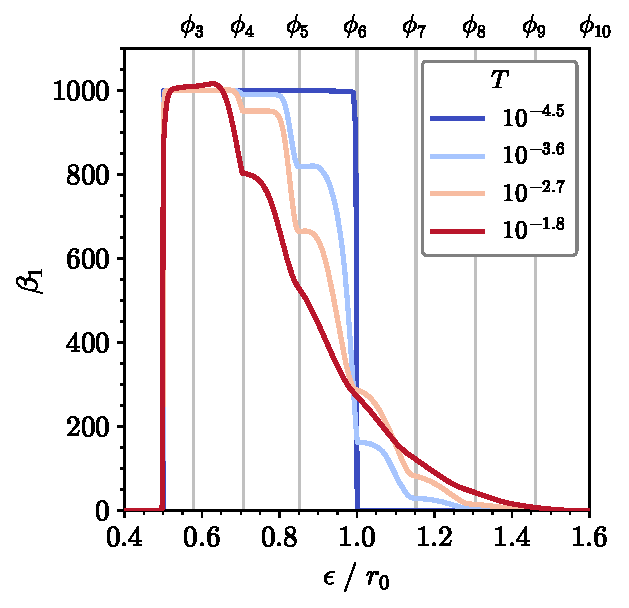
\includegraphics[width=\textwidth]{./figures/ph/tri_raft_beta1_full.pdf}
         \caption{}
         \label{fig:trbettia}
     \end{subfigure}
     \hfill
     \begin{subfigure}[b]{0.45\textwidth}
         \centering
         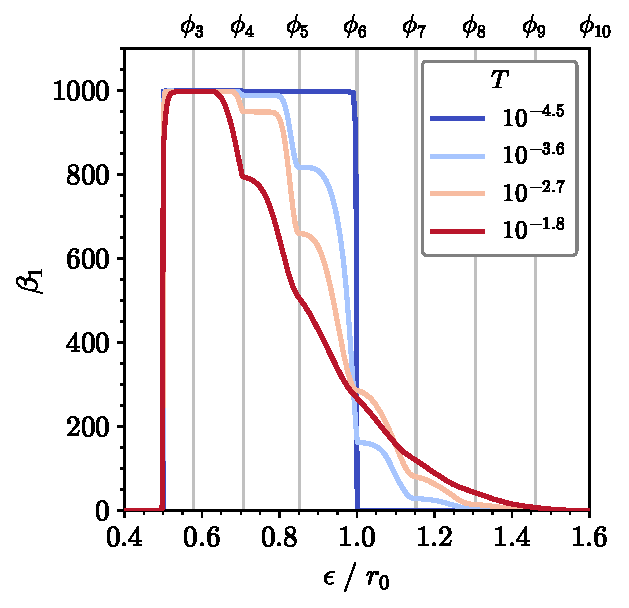
\includegraphics[width=\textwidth]{./figures/ph/tri_raft_beta1_cut.pdf}
         \caption{}
         \label{fig:trbettib}
     \end{subfigure}

	\caption{Evolution of the first Betti number with filtration for triangle rafts at different levels of disorder. In panel (a) the calculation includes all cycles, whereas panel (b) includes only the $1000$ most persistent cycles. The circumradii of regular polygons with $k$ vertices, $\Phi_k$, are indicated by vertical grey lines.}
	\label{fig:trbetti}
\end{figure}

As is now expected, $\beta_1$, rises very sharply from $0\rightarrow 1000$ at $\epsilon=0.5r_0$, as the first cycles form at half the mean bond distance.
The value of $\beta_1$ must then decay to zero in the limit of $\epsilon\rightarrow \infty$, but the form of the curve varies with the system temperature.
At the lowest temperature, which is primarily a hexagonal lattice, the function is almost a step function at $\epsilon=1.0r_0$, but as the temperature increases, and more diverse ring sizes are incorporated, the curve broadens and smoothens.
Even for the highest temperature, the decay in $\beta_1$ is not however smooth, but a series of stepwise decrements.
These decrements align very closely to the values of the circumradii of $k$\--polygons with unit edge lengths, $\Phi_k$, given in table \ref{tab:circumradii}.
As discussed in the previous section, $\Phi_k$ represents the upper bound on the death value for a $k$\--polygon in $B_1$, for triangle rafts. 
Any deviations from regularity therefore act to reduce the lifetime.
This largely explains the full behaviour of the curves in figure \ref{fig:trbetti}.
The discontinuities represent changes between successive $k$\--cycles dying, with the broadening of the curve indicative of the increasing variety of $k$ values and the smoothening the increased polygon distortion \-- both of which increase with temperature.
It is interesting to note that the secondary cycles do not seem to affect the Betti numbers to a large degree, as evidenced by the similarity of figures \ref{fig:trbettia} and \ref{fig:trbettib}.
Only at the highest temperature is there a detectable presence in the region between $\epsilon=0.5\rightarrow0.7r_0$.
This is because these species are so relatively short\--lived and spread throughout the filtration range, that at any filtration value they add a virtually insignificant contribution to the total. 


\begin{figure}[tb]
	\centering
     
     \begin{subfigure}[b]{0.48\textwidth}
         \centering
         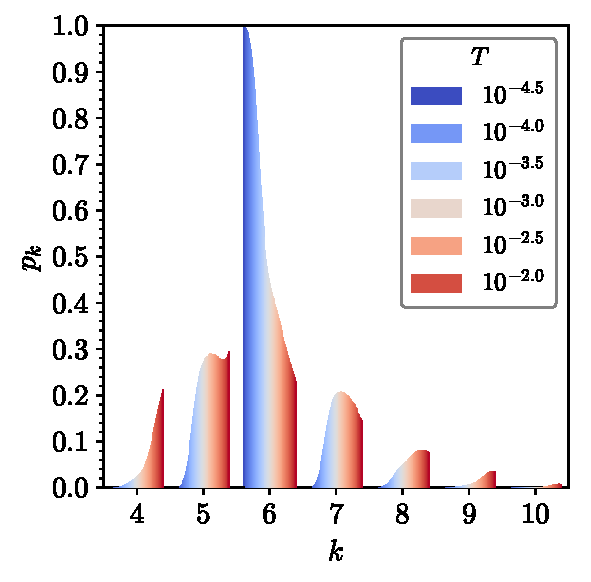
\includegraphics[width=0.87\textwidth]{./figures/ph/tr_pk_ph.pdf}
         \caption{Cycle statistics}
         \label{fig:trpkpha}
     \end{subfigure}
     \hfill
     \begin{subfigure}[b]{0.48\textwidth}
         \centering
         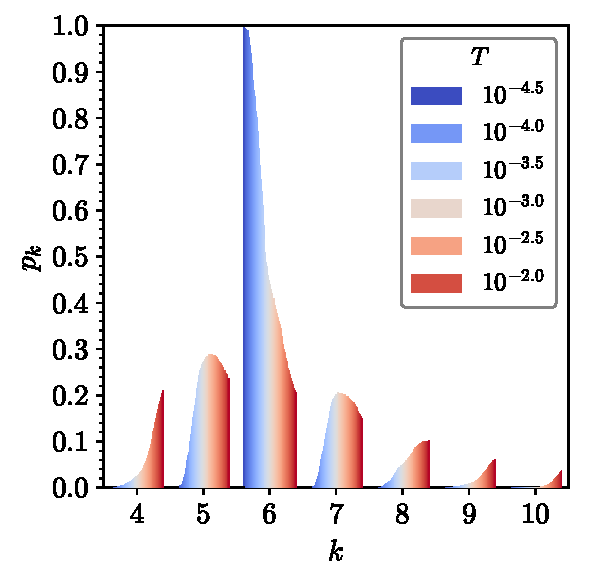
\includegraphics[width=0.87\textwidth]{./figures/ph/tr_pk_true.pdf}
         \caption{Ring statistics}
         \label{fig:trpkphb}
     \end{subfigure}

     \vspace{2mm}     
      \begin{subfigure}[b]{0.96\textwidth}
         \centering
         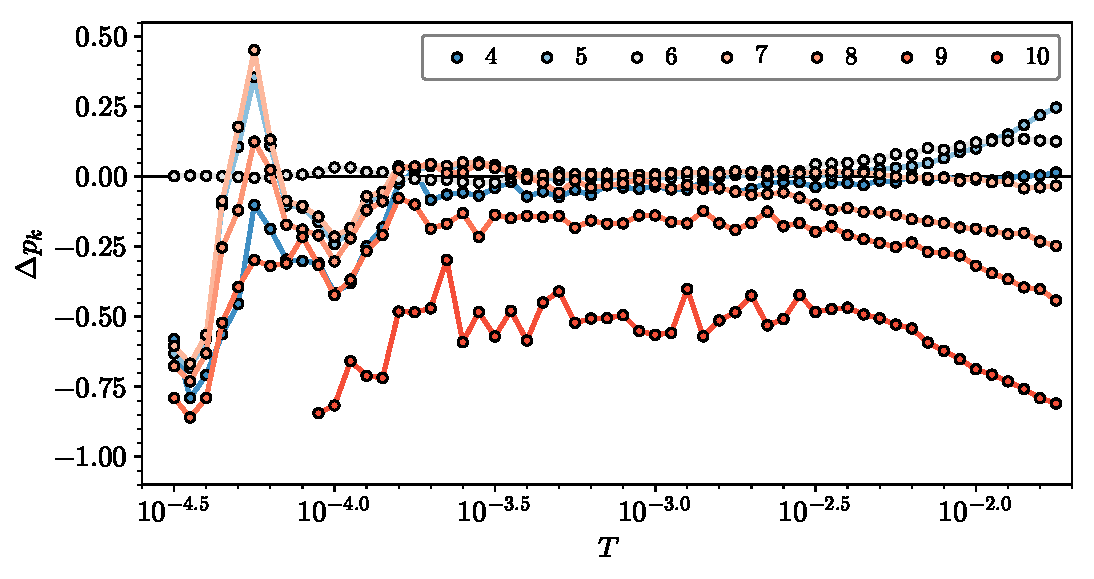
\includegraphics[width=0.87\textwidth]{./figures/ph/tr_delta_pk.pdf}
         \caption{}
         \label{fig:trpkphc}
     \end{subfigure}

	\caption{Comparison of the $k$\--cycle statistics, panel (a), against the ring statistics, panel (b), in triangle rafts across different levels of disorder. Panel (c) gives a direct comparison between the two.}
	\label{fig:trpkph}
\end{figure}


With this logic, it should be possible to extract the cycle statistics, which will be denoted $p_k$, in analogy with ring statistics.
To do so, one simply needs to calculate:
\begin{equation}
	p_k = \beta_1\left(\Phi_k\right)-\beta_1\left(\Phi_{k-1}\right),
\end{equation}
and normalise across all $k$ values.
The cycle statistics from this process are given in figure \ref{fig:trpkpha}, which can be considered in reference to the ring statistics in figure \ref{fig:trpkphb}.
In addition, the comparative measure,
\begin{equation}
	\Delta p_k = \frac{p_k^\text{cycles}-p_k^\text{rings}}{p_k^{\text{rings}}},
\end{equation}
is given in figure \ref{fig:trpkphc}.
To a first approximation the agreement is very good, particularly for the ring sizes close to $k=6$, at modest temperatures.
This means that the cycles computed via persistent homology agree well with the primitive rings in the system, taking account for the approximate method to calculate $k$\--cycles.
Deviations are accentuated at very low temperature, when the absolute ring statistics of non\--six rings are small, or at high temperatures, when rings are increasingly distorted.
For example, it is clear that $p_{10}$ is systematically underestimated from cycles across the whole temperature range.
In addition, the statistics of smaller rings ($k\leq6$) are overestimated and larger rings ($k\geq 8$) underestimated increasingly at higher temperatures.

The reason for this is that when large rings become sufficiently distorted, for instance becoming very elongated or even slightly non\--convex, the cross ring distances become sufficiently small that they die much earlier than expected.
Examining the polygons in figures \ref{fig:b3a} and \ref{fig:b4a}, and referring again to table \ref{tab:circumradii}, one can see that almost all of these examples would be classified as being of a smaller cycle size than they are in reality, when examining the death values.
Considering all these factors, overall in two dimensions, for triangle rafts, it is reasonable to conclude that the cycles found from persistent homology are in almost exact accordance with the primitive rings in the system.

\section{Persistent Homology with CRNs}

The results of persistent homology with triangle rafts led to a well defined band structure in the persistence diagrams, as a consequence of the tightly controlled ring geometries.
This structure is not always observed in simulations, for example with Cu\--Zr alloys and high density molecular liquids \cite{Hiraoka2016,Onodera2019}.
In these cases, more diffuse diagrams are found, which naturally accompanies the increase in degrees of freedom in such systems.
The triangle raft algorithm is unable to directly reproduce these effects in two dimensions, owing to the innate rigidity of the model.
However, this can be achieved with another algorithm developed in this thesis, namely bond switching \ref{s:bondswitch}.
In bond switching, the potential model allows for greater freedom in the bond lengths and angles, and the process of randomising an existing lattice (as opposed to building an random ring structure sequentially) allows configurations with a greater range of ring sizes, and a greater level of ring disorder, to be realised.

Therefore, in this section, persistent homology analysis will be performed on the configurations generated from bond switching, applying the information learned from analogous calculations on triangle rafts.
The specific systems studied will be a subset of those from chapter \ref{ch:generalnetworks}, namely those at two different bond stretching and angle force constant ratios of $\fk_r/\fk_\theta=16,4$, with convexity maintained.
The persistence diagrams and change in Betti numbers will be investigated for these systems, and the effect of the potential model highlighted.
In addition, the results will be contrasted with those of triangle rafts.
Again calculations were performed with the GUDHI library \cite{gudhi}, and birth and death filtration values are given with reference to the equilibrium bond length, $r_0$.

\subsection{Persistence Diagrams}

The persistence diagrams for bond switching configurations generated with the two potential models are given in figure \ref{fig:bspd}.
Figures \ref{fig:bspda}\--\ref{fig:bspdd} pertain to the force constant ratio $\fk_r/\fk_\theta=16$ and figures \ref{fig:bspde}\--\ref{fig:bspdh} at $\fk_r/\fk_\theta=4$.
For both models, four different $p_6$ values were selected, corresponding to four increasing levels of disorder.
The initial impression may be that the persistence diagrams look very different from those of triangle rafts in figure \ref{fig:trpd}, but closer inspection reveals this is not the case, and they share many of the same characteristics.

A key reason for these apparent differences is that the bond lengths have inherently more flexibility in the case of bond switching than triangle rafts.
As such, any similar features will appear much broader, but retain similar structural origins.
For example, the $B_1$ band is present in all the diagrams in figure \ref{fig:bspd}, centred around $b=0.5r_0$.
The difference is that at low levels of disorder  (see for example figures \ref{fig:bspda}\--\ref{fig:bspdb}), one can clearly see distinct ``spots'' in $B_1$, which are present in figure \ref{fig:trpd} but harder to detect due to the narrowness of the band.
The upper limits of these spots correspond well with the circumradii in table \ref{tab:circumradii} \ie{} they are related to the occurrence of specific $k$\--cycles.
At higher disorder these spots begins to coalesce, as in figure \ref{fig:bspdc}, before fully combining to form a single high density feature, as in figure \ref{fig:bspdd}.

\begin{figure}[tbp]
	\centering
     
      \begin{subfigure}[b]{0.40\textwidth}
         \centering
         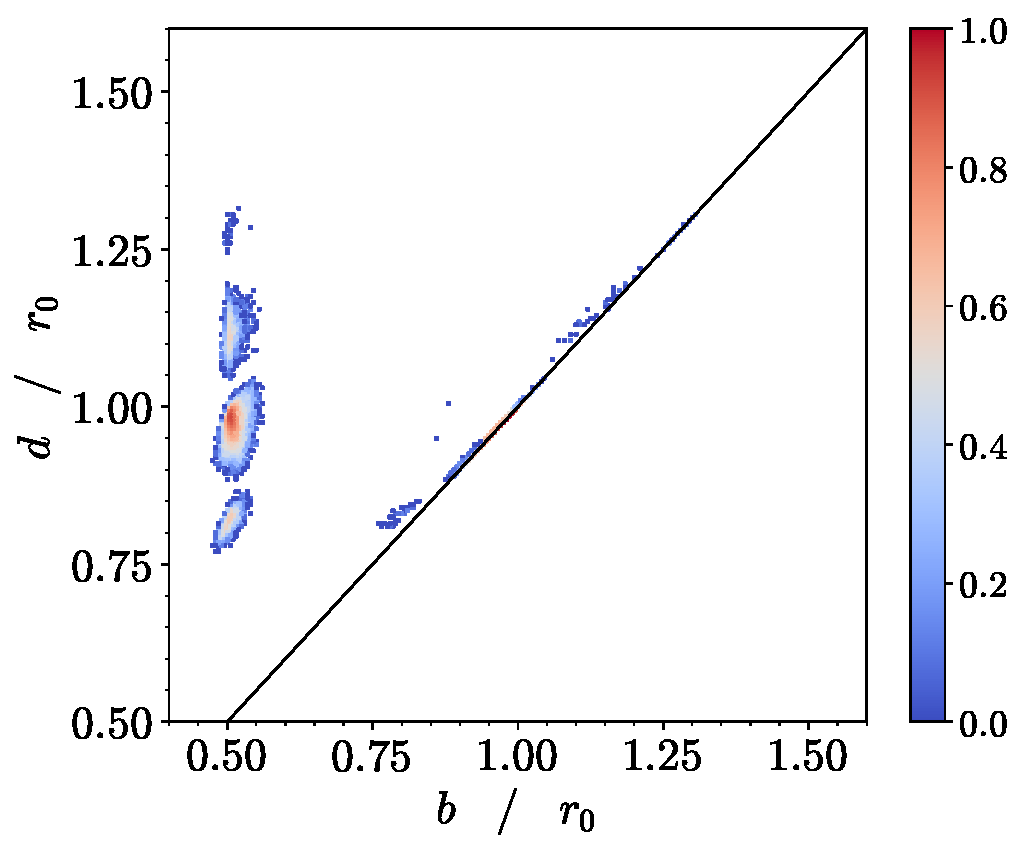
\includegraphics[width=\textwidth]{./figures/ph/t_k16_399_bs_pd.pdf}
         \caption{$\fk_r/\fk_\theta=16$, $p_6=0.890$} %399
         \label{fig:bspda}
     \end{subfigure}
     \hspace{1cm}
        \begin{subfigure}[b]{0.40\textwidth}
         \centering
         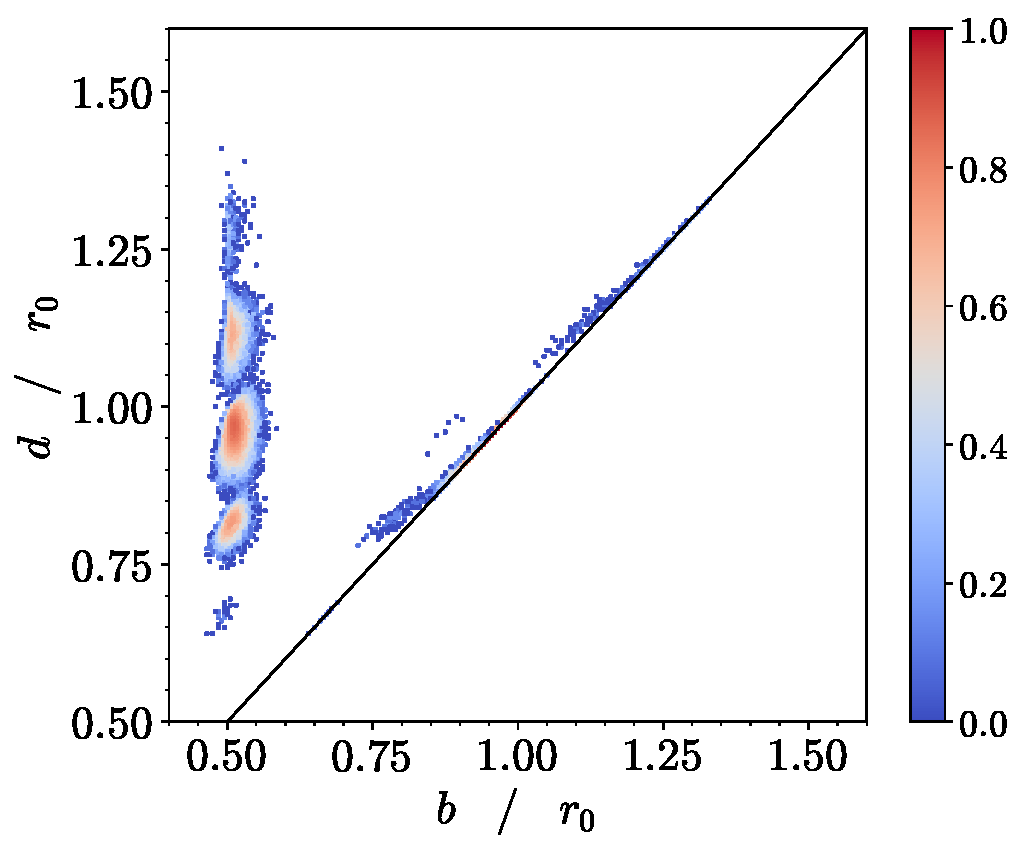
\includegraphics[width=\textwidth]{./figures/ph/t_k16_301_bs_pd.pdf}
         \caption{$\fk_r/\fk_\theta=16$, $p_6=0.666$}% 301
         \label{fig:bspdb}
     \end{subfigure}
     
        \begin{subfigure}[b]{0.40\textwidth}
         \centering
         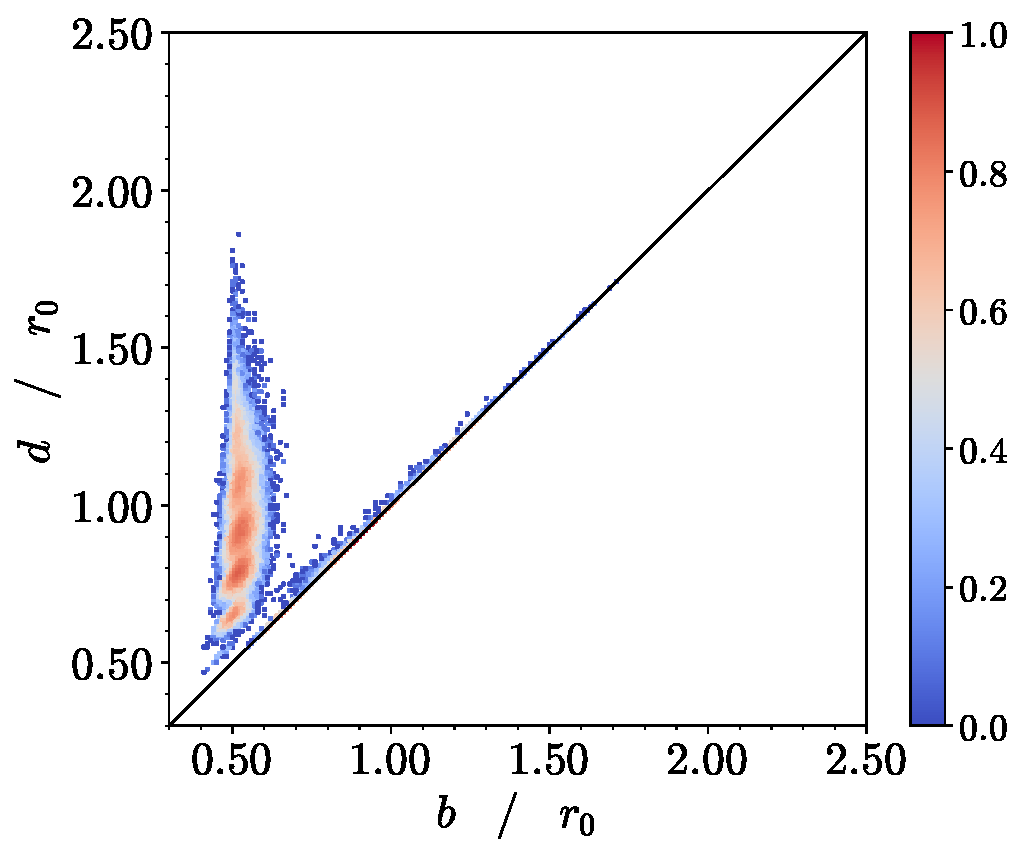
\includegraphics[width=\textwidth]{./figures/ph/t_k16_231_bs_pd.pdf}
         \caption{$\fk_r/\fk_\theta=16$, $p_6=0.332$}% 231
         \label{fig:bspdc}
     \end{subfigure}
     \hspace{1cm}
      \begin{subfigure}[b]{0.40\textwidth}
         \centering
         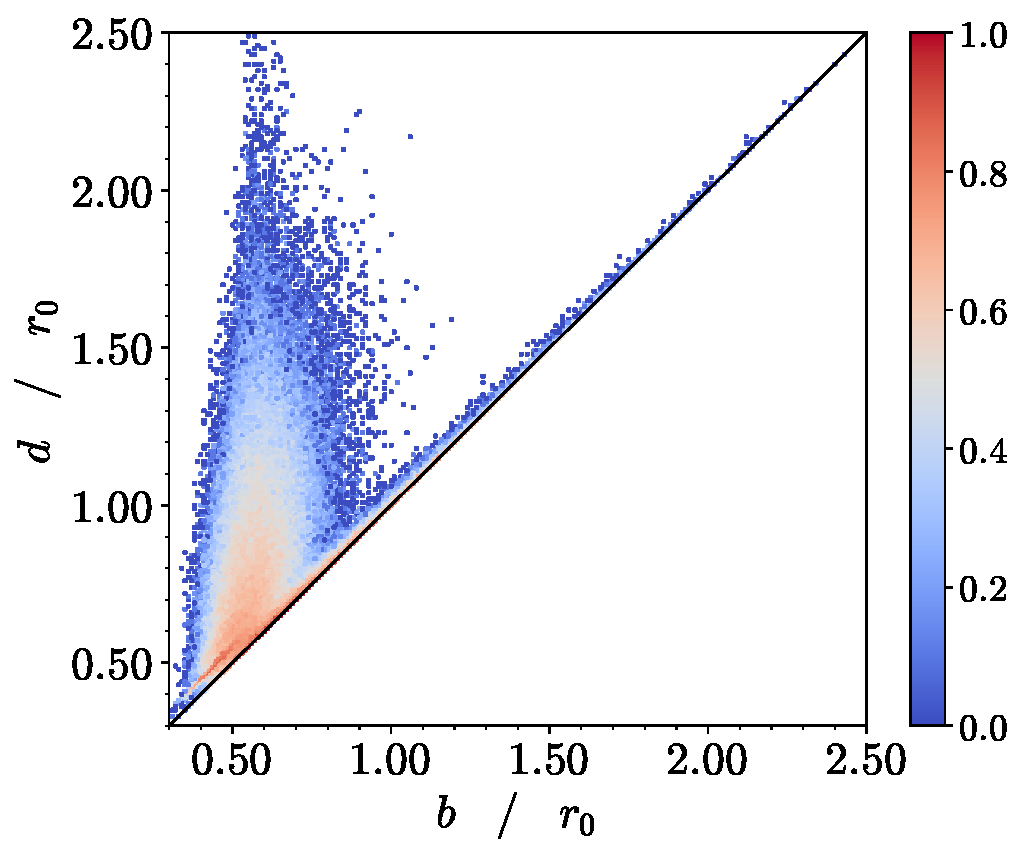
\includegraphics[width=\textwidth]{./figures/ph/t_k16_0_bs_pd.pdf}
         \caption{$\fk_r/\fk_\theta=16$, $p_6=0.164$}% 0
         \label{fig:bspdd}
     \end{subfigure}


	\begin{subfigure}[b]{0.40\textwidth}
         \centering
         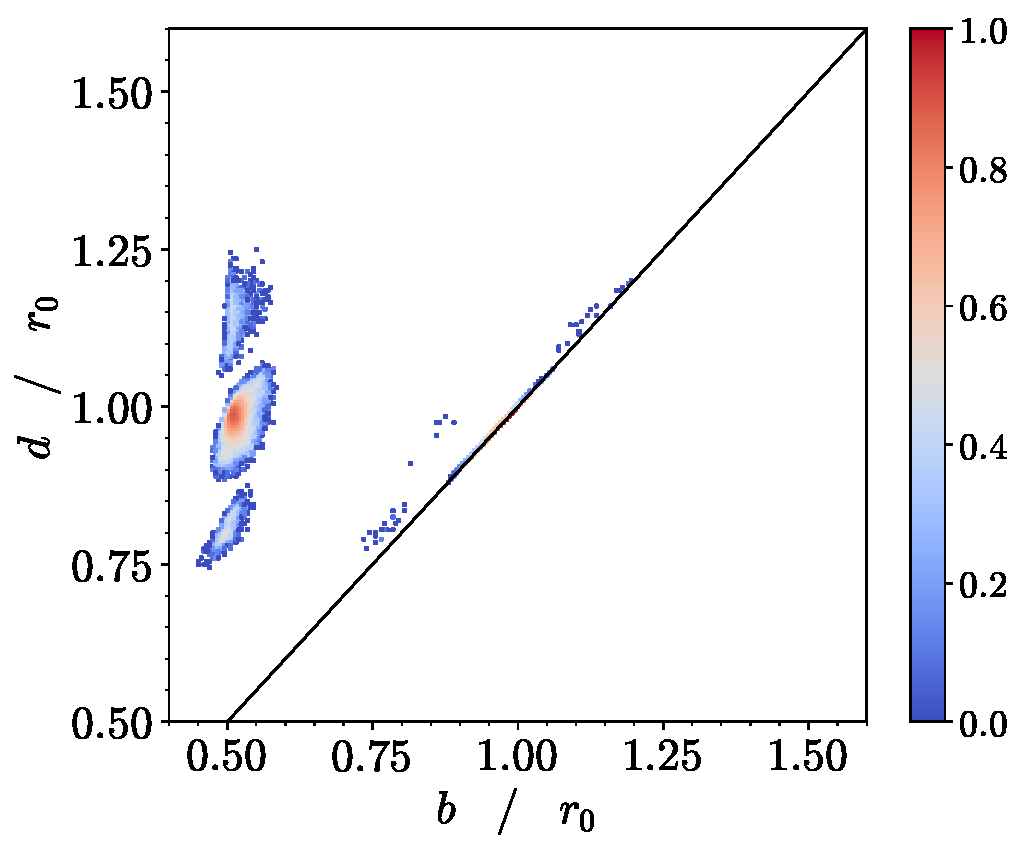
\includegraphics[width=\textwidth]{./figures/ph/t_k4_399_bs_pd.pdf}
         \caption{$\fk_r/\fk_\theta=4$, $p_6=0.943$}% 399
         \label{fig:bspde}
     \end{subfigure}
     \hspace{1cm}
        \begin{subfigure}[b]{0.40\textwidth}
         \centering
         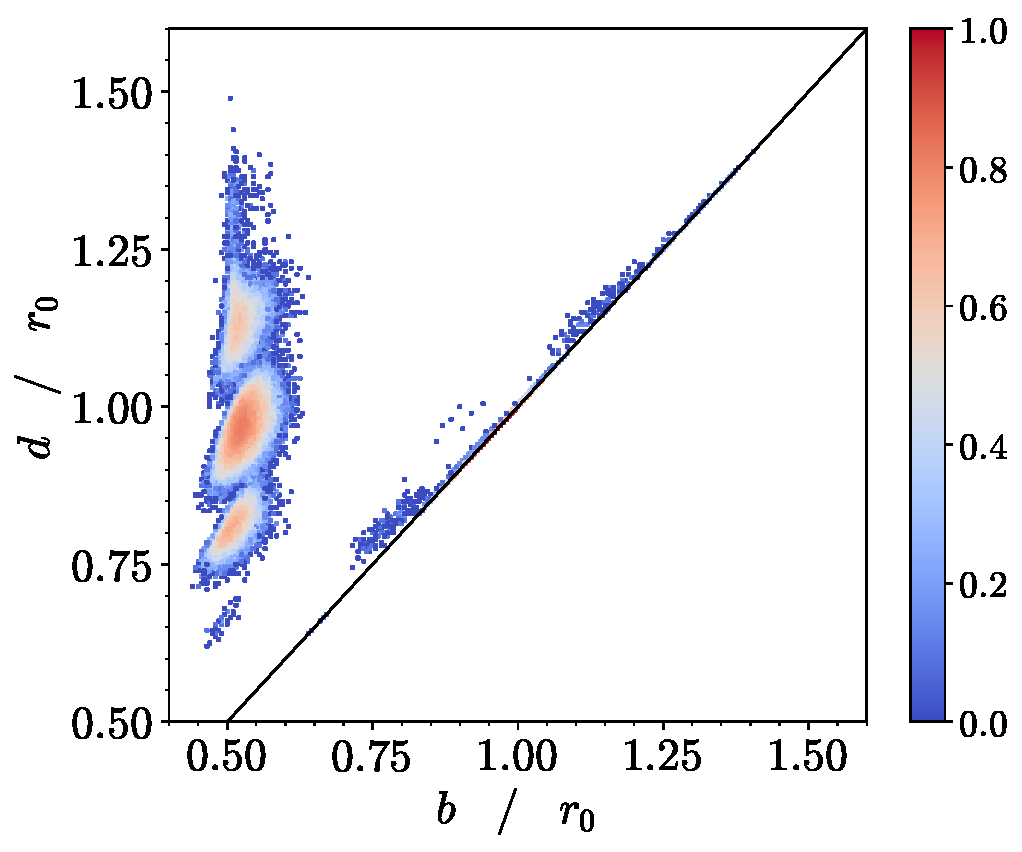
\includegraphics[width=\textwidth]{./figures/ph/t_k4_257_bs_pd.pdf}
         \caption{$\fk_r/\fk_\theta=4$, $p_6=0.662$}% 257
         \label{fig:bspdf}
     \end{subfigure}
     
        \begin{subfigure}[b]{0.40\textwidth}
         \centering
         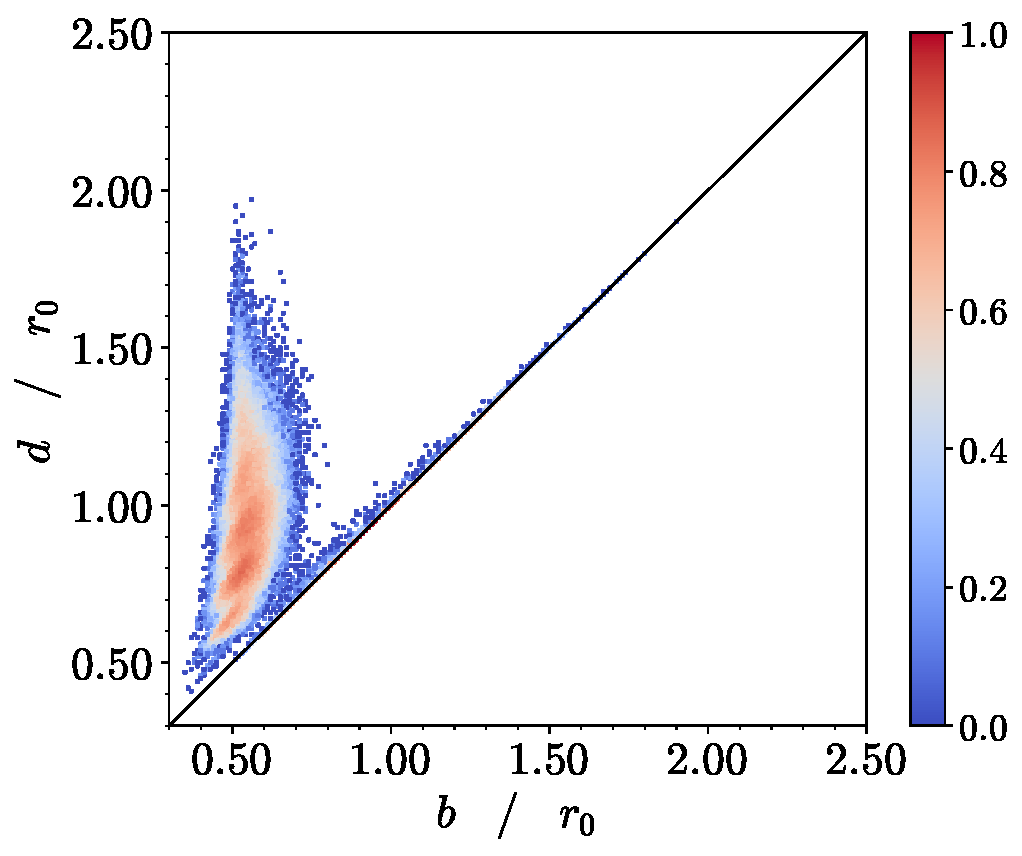
\includegraphics[width=\textwidth]{./figures/ph/t_k4_189_bs_pd.pdf}
         \caption{$\fk_r/\fk_\theta=4$, $p_6=0.332$}% 189
         \label{fig:bspdg}
     \end{subfigure}
     \hspace{1cm}
      \begin{subfigure}[b]{0.40\textwidth}
         \centering
         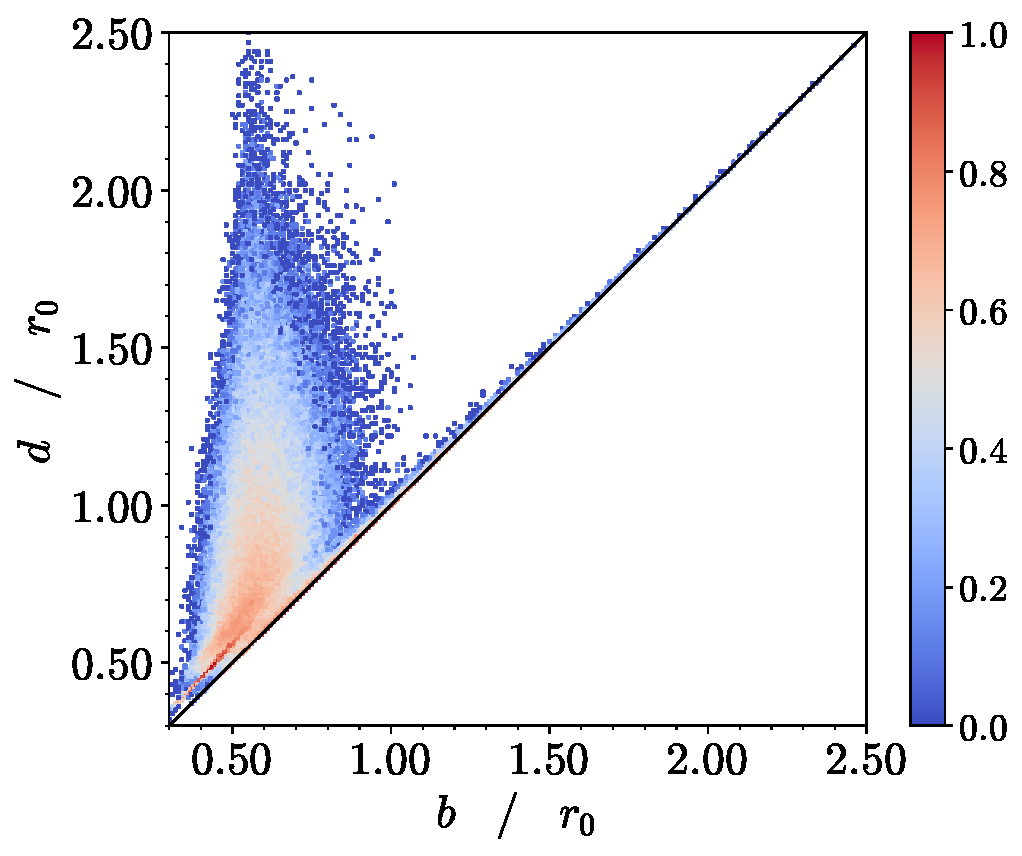
\includegraphics[width=\textwidth]{./figures/ph/t_k4_0_bs_pd.pdf}
         \caption{$\fk_r/\fk_\theta=4$, $p_6=0.163$}% 0}
         \label{fig:bspdh}
     \end{subfigure}
     
	\caption{Persistence diagrams for configurations from bond switching, at different bond stretch/angle force constants and $p_6$ (as indicated in captions).}
	\label{fig:bspd}
\end{figure}

This final diagram can be considered ``typical'' of a highly disordered amorphous or liquid state \cite{Hiraoka2016,Onodera2019}.
By using the bond switching method, it is clear however that this originates from the broadening and aggregation of features relating to individual cycle sizes.
Other bands in the persistence diagram are also detectable, in particular $B_3$, but largely only at higher $p_6$ values. 
This is because these bands only occur when there are well defined large cycles.
In bond switching, although there are primitive rings which are very large, these can become so distorted that they are not calculated as a single persistent cycle, but rather multiple smaller cycles.
This precludes the formation of significant higher order bands as seen in triangle rafts. 

%Other bands in the persistence diagram are also detectable, in particular $B_3$, but largely only at higher $p_6$ values. 
%This is because these bands only occur when there are well defined large cycles.
%In bond switching, although there are primitive rings which are very large, these can become so distorted that they are not calculated as a single persistent cycle, but rather multiple smaller cycles.
%This precludes the formation of significant higher order bands as seen in triangle rafts. 
%There is however one band which develops that was not previously observed in triangle rafts, which is the small intense region in figures \ref{fig:bspdd} and \ref{fig:bspdh} below $b=0.5$.
%It will be shown in the following section that this is due to the presence of fleeting secondary cycles.

As for the comparison between the different potential models, the effect of changing the force constant ratio appears relatively small.
By comparing the persistence diagram of similar $p_6$ values, one can see there is a general broadening of the regions corresponding to each cycle size on reducing the bond stretch to angle ratio.
The rationale for this trend is the same as for increasing temperature - that increasing the variation in nearest\--neighbour interatomic distances comes with associated variation in the values at which cycles are born and die.
The difference between potential models naturally becomes less pronounced as disorder increases, and the Monte Carlo temperature is effectively infinite, such that the final diagrams, figures \ref{fig:bspdd} and \ref{fig:bspdh}, are almost identical.
In these diagrams, the gradient of the $B_1$ line appears to become progressively shallower, driven by the decreasing birth value of smaller cycles.
This is likely because the birth filtration value of a cycle depends on the final 1\--simplex to form.
As a cycles becomes larger, the probability that all constituent 1\--simplices will have filtrations less that $b=0.5r_0$ becomes increasingly unlikely compared to smaller cycles.
The result of this is that smaller cycles, with lower death values, can also have progressively lower birth values, leading to the perceived tilting of the $B_1$ band.

\subsection{Evolution in Betti Numbers}

The first Betti number, $\beta_1$, can again give insight into the cycle structure in configurations generated from bond switching.
Figures \ref{fig:bsbettia} and \ref{fig:bsbettib} show the evolution in $\beta_1$ with $\epsilon$ for the two variations in potential, where $\fk_r/\fk_\theta = 16,4$.
In all cases configurations contain 1024 rings, averaged over 100 samples. 
For both potentials, at the two higher $p_6$ values, the curves exhibit similar behaviour to those from triangle rafts.
Around $\epsilon=0.5r_0$, 1024 cycles form, corresponding to the primitive rings in the system, before decaying in a stepwise fashion at filtration values corresponding to the regular $k$\--polygon circumradii.
However, at the lower $p_6$ values, the curves become smooth and the maximum decreases to around half its original value.
As there remain the same number of primitive rings, the implication of the maximum reducing is that some cycles die before others are even born and they never coexist.
This in turn means that all these rings are not detectable on the same length scale.

The final broad distribution resembles closely that of previous studies of random structures \cite{Nakamura2015}.
This can therefore be considered characteristic of a highly amorphous (approaching liquid) disordered limit.
As mentioned for the corresponding persistence diagrams, this results from the large variation in bond length and angle distributions %\davidnote{Todo: discuss if it would be useful to include histograms of the bond lengths/angles in all this discussion.}.
Once again, the effect of changing the force constant ratio is weak, with some broadening observed for $\fk_r/\fk_\theta=4$ over $\fk_r/\fk_\theta=16$ at higher $p_6$ values.

\begin{figure}[tb]
	\centering
     
      \begin{subfigure}[b]{0.45\textwidth}
         \centering
         \includegraphics[width=\textwidth]{./figures/ph/bs_k16_beta1_cut.pdf}
         \caption{$\fk_r/\fk_\theta=16$}
         \label{fig:bsbettia}
     \end{subfigure}
     \hfill
     \begin{subfigure}[b]{0.45\textwidth}
         \centering
         \includegraphics[width=\textwidth]{./figures/ph/bs_k4_beta1_cut.pdf}
         \caption{$\fk_r/\fk_\theta=4$}
         \label{fig:bsbettib}
     \end{subfigure}

	\caption{Evolution of the first Betti number with filtration for bond switching configurations at different levels of disorder and two different potential models (as indicated in captions).}
	\label{fig:bsbetti}
\end{figure}

\section{Evaluation of Persistent Homology}

Having investigated the results of persistent homology calculations for range of \td{} systems, an attempt will be made to draw conclusions on the utility of persistent homology in the characterisation of \td{} materials and more complex atomic systems.
To begin with, the success of persistent homology is evaluated in comparison to other, more established, analysis methods.
For systems with relatively rigid geometries, persistence diagrams have proved effective in showing the evolution in structure through the band structure.
On the one hand, these diagrams can be considered to contain more information than other measures such as RDFs, as the interaction distances are already partitioned into increasing nearest\--neighbour contributions.
On the other hand, the distances conveyed by the filtration value can be viewed as less intuitive than other real\--space methods, being related to the circumcircles of variously sized simplices.

Nevertheless, presenting these data through the Betti numbers does allow a good estimation of the ring statistics in the system.
The natural analogue of this would be integrating under successive peaks in the RDF to extract coordination numbers.
In this case persistent homology does give access to clear information which is hard to extract otherwise.
It is worth remembering that the samples studied in this chapter were computationally generated, and the ring structure is readily available.
However, experimental images are often less well resolved, possibly containing areas which could not be fully imaged.
Persistent homology can provide a computationally tractable way of obtaining the ring structure, which must otherwise be achieved by a brute force path search.
The benefits are more nuanced than simple speed concerns.
By definition, persistent homology considers cycles appearing at different length scales, and so one can separate the rings trivially from large holes in defective samples.

When materials have more flexibility, the efficacy of persistent homology is less clear cut.
At relatively low levels of disorder the metrics described above still apply, but in highly amorphous systems, the cycles no longer become reflective of the primitive ring structure.
%Rather, the persistence diagram adopts a more generic and diffuse form.
Whilst the relative flexibility in the atomic potential is detectable through broadening of features, it is not clear that it is quantifiable.
Furthermore, there is no evidence as yet that persistent homology is able to capture information on the medium range ring order, as for instance provided by the assortativity or \aw{} parameter.
In fairness to the method, almost by definition, other classical measures such as the RDF equally lose information as structure is lost.
%In the case of persistent homology, it is not yet clear that anything ``more'' is available in this situation.

Based on these \td{} analyses, there is certainly scope for further application of persistent homology to \thd{} systems, as has been attempted in previous studies.
The question is whether the same insight can be gained, as there is a less well defined ring structure.
There are also additional complications with increasing dimensionality, in that the next homology group is also accessible.
In the \td{} case, the focus was on cycles which were filled with triangles, but in \thd{} there are also voids which are filled with tetrahedra.
The advantage of persistent homology is that these different groups are trivially separable, and it may be that in \thd{} systems that the voids carry more structural significance.
However, one further potential downside is that while real\--space data is becoming widespread for \td{} systems, direct imaging is less feasible for \thd{} structures.
This would limit persistent homology calculations to computational systems, which adds another layer of abstraction when comparing to experimental results.
%Irrespective of this added complexity, the \td{} case has at least demonstrated how physical structure can be related to persistent topological features.

Overall, there is cause for cautious optimism for the use of persistent homology as another tool in the characterisation of amorphous materials.
It is certainly true that to the trained eye, a persistence diagram of a crystal, amorphous material and liquid are easily identifiable, and information on the ring structure may also be gleaned. 
Once the principle is understood, there is no more inherent difficulty in interpreting such diagrams than RDFs, structure factors or any other traditional measure.
In addition, the use of persistent homology is by no means limited to chemical systems, and it may be that improvements in other fields will allow a novel interpretation of the structure of atomistic configurations.
   
\section{Chapter Conclusions}

Persistent homology, a tool from topological data analysis, has been applied to the study computational configurations of \td{} materials.
These were generated using methods described elsewhere in this thesis, namely triangle rafts and bond switching.
Whilst the analyses of the two systems displayed similarities, the differences in the underlying constraints manifested in the persistence diagrams and Betti numbers.
The relatively constrained triangle rafts showed well defined bands in the persistence diagrams, which were traced to successive nearest\--neighbour interactions, which broadened as ring disorder increased.
The introduction of new ring sizes could also be quantified by plotting the Betti numbers with filtration value.
On the other hand, the configurations from bond switching displayed similar features, but these quickly aggregated with increased disorder to make quantifying the structure more difficult.

In general, persistent homology has been shown to have potential as an investigative tool for studying \td{} materials, where persistent features can be explicitly linked to atomic interactions.
It remains an open question whether similar links can be developed for use with \thd{} systems, particularly in experiment when real\--space data is less readily available.
